\chapter{给定模型下的规划}
\label{chap:rl-planning}

第~\ref{chap:rl-overview}~章用随机滑移的网格说明了为何要比较动作的长期后果，也证明了回报期望满足Bellman递推。本章把问题进一步收紧：假设导航模型已经给出，我们能够查询每个合法动作会把机器人带向何处、得到什么奖励。于是待求的对象不再是“环境规律是什么”，而是“怎样利用已知规律算出一份好策略”，这类在给定模型上求解最优或近似最优行为的工作统称为规划（planning）。

即使规律全部已知，规划仍有计算上的困难。一次查询只涉及一个状态动作，可一份策略必须应对机器人后续可能到达的许多状态；把所有后果枚举出来、为每个状态保存价值、以及把价值算到所需精度，都要消耗计算、存储与查询资源。本章的主线就是考察：在给定的资源预算下，怎样把“一步查询”组织成对整段未来的评价。

在进入方法前，还要先弄清“模型已经给出”到底允许我们取得什么答案，因为不同的允许方式对应不同的算法与代价。给定一个后继价值估计$v$，要比较当前动作，需要计算当步期望奖励与折扣后继价值之和。\term{精确期望访问}（exact expectation access）允许直接计算
$R(s,a)+\gamma\sum_{s'}T(s'\mid s,a)v(s')$；网格模型若明确列出了向前和向两侧滑移的全部概率，就能按概率逐项加权求和。\term{生成模型访问}（generative model access）则弱得多：它只允许指定任意合法的$(s,a)$，再取得一个独立样本$(r,s')\sim p(\cdot,\cdot\mid s,a)$，相当于反复调用一个模拟器。重复同一查询可能返回不同后果，规划器只能用样本均值估计上述期望。

生成模型无须公开概率表，也不要求规划器先从起点走到$s$；它提供的是从指定查询点正确采样的能力。因此，模型准确并不意味着有限次查询已经给出准确期望。本章把两种接口都作为给定资源，在各方法中分别说明所需能力。尤其不能把真实机器人的交互默认成生成模型：机器人通常只能从当前位置继续行动，不能任意重置到待查状态。后面的稀疏采样规划依赖这种指定查询点的能力\scite{rl2-kearns2002-sparse}

我们先沿用前章的有限折扣MDP：状态、动作集合有限，每个$\mathsf A(s)$非空，$|r_t|\leq R_{\max}$，且$0\leq\gamma<1$。奖励$r_t$仍按执行$a_t$的时刻编号，价值和策略性能仍是未归一化折扣回报。前章的有界回报结论于是给出$|V^\pi(s)|\leq V_{\max}:=R_{\max}/(1-\gamma)$。讨论有限时域、成本最小化或平均奖励时，我们会在当地重新规定目标，避免把这些设定混入折扣结论。

在这些条件下，本章按“预算从充足到紧张”的顺序组织求解方式。若计算与存储都充足，Bellman动态规划逐状态使用递推，全局优化则同时约束所有状态动作；这是两条求解同一目标的一般精确路线。若动力学、成本或子任务之间还存在额外结构，有时能显著减少精确求解所需的未知量或动作比较，但每一种简化都必须逐项验证其条件是否成立。若状态数或搜索树仍超出预算，还剩两条近似路线：只为当前状态展开局部后果，或保存一份跨状态复用的近似价值；局部搜索又可以借助这份近似价值评估未展开的未来，因此两类近似能够配合。图~\ref{fig:rl-planning-map}~展示的正是这些求解方式及其联系，后文再用误差和资源要求逐一比较它们。

\begin{figure*}[htbp]
  \centering
  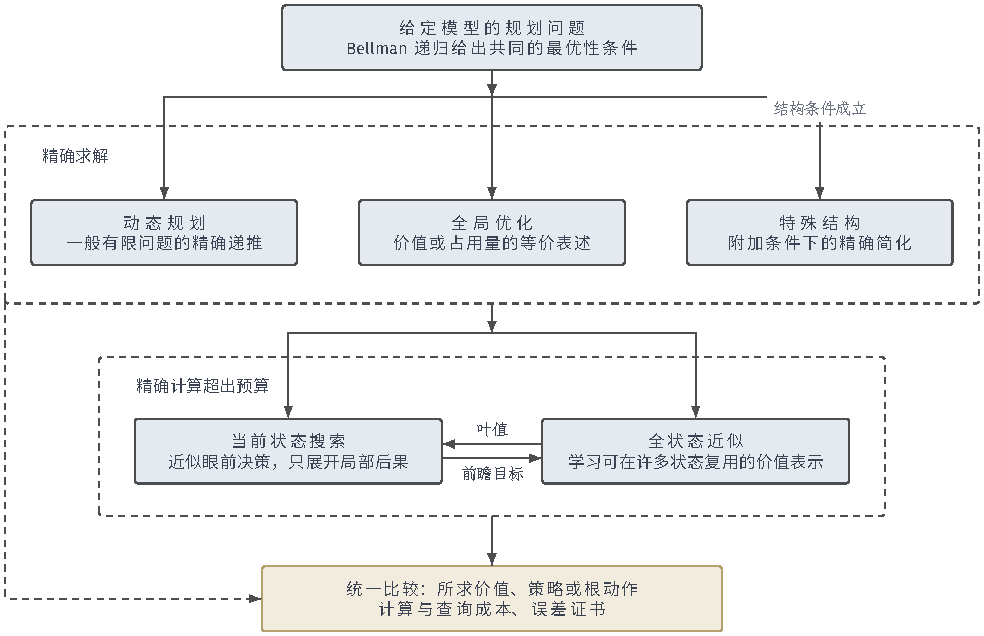
\includegraphics[width=166.617mm]{figures/07-reinforcement-learning/01-problems-and-solving/tikz/rl-planning-map.pdf}
  \caption{给定模型时的规划方法关系。动态规划与全局优化是一般精确路线；特殊结构只在附加条件成立时给出精确简化。精确计算超出预算后，可以近似当前决策或构造全状态近似，二者可通过叶节点价值与前瞻目标结合。}
  \label{fig:rl-planning-map}
\end{figure*}

% Outline: 2.1
\section{Bellman动态规划}
\label{sec:rl-planning-dp}

在网格的一个岔路口，若已经知道各后继状态的价值，就能用“当步奖励加折扣后继价值”比较各个合法方向，而不必把这些方向之后的全部轨迹重新枚举一遍。动态规划（dynamic programming）反复利用这种一步分解：先求出较短未来的价值，再用它算出较长未来的价值，逐步得到原先难以直接计算的长期价值。本节分三步走：先固定一条动作规则、只算遵从它的后果（策略评价），再用评价结果比较其他动作（策略改进），最后把动作选择直接并入价值更新（价值迭代）。

% Outline: 2.1.1
\subsection{策略评价}
\label{sec:rl-planning-evaluation}

给定平稳策略$\pi$，策略评价要算的是从每个状态出发遵从它的$V^\pi$，这一步并不重新选择动作，动作概率完全由给定的$\pi$决定。为把前章的Bellman关系整理成可以求解的线性方程，先把当步奖励和转移概率都按$\pi$平均：
\[
 r^\pi(s)=\sum_a\pi(a\mid s)R(s,a),\qquad
 T^\pi(s,s')=\sum_a\pi(a\mid s)T(s'\mid s,a).
\]
这样得到的$r^\pi$是按$\pi$行动时的当步期望奖励，并非一次模拟实际拿到的数值；$T^\pi$描述“遵从$\pi$时”下一状态的分布，它把动作选择的随机性和环境转移的随机性合在了一起。在精确期望接口下，按状态排列的$\bm r^\pi$和$\bm T^\pi$都可以直接算出，整张表里唯一未知的就是价值向量。令$\bm v^\pi$的$s$坐标为$V^\pi(s)$，Bellman方程便写成
\begin{equation}
 \bm v^\pi=\bm r^\pi+\gamma\bm T^\pi\bm v^\pi,\qquad
 (\bm I-\gamma\bm T^\pi)\bm v^\pi=\bm r^\pi.
 \label{eq:rl-planning-linear-evaluation}
\end{equation}
矩阵$\bm T^\pi$非负且每行之和为1，其无穷范数（最大绝对行和）为1。这意味着$\|\gamma\bm T^\pi\|_\infty=\gamma<1$：每多向前递推一层，未来的贡献就要再打一次折扣。于是矩阵几何级数$\sum_{k\geq0}\gamma^k(\bm T^\pi)^k$收敛到$(\bm I-\gamma\bm T^\pi)^{-1}$，评价方程因而有唯一解，而且可以直接写出来。矩阵范数和逆矩阵级数的结论可参考\BookChapterRef{chap:linear-algebra-and-matrix-analysis}{卷1《数学准备：计算、分析与几何》中“线性空间”章}。这个级数解还有一层直观含义：把它乘开后，第$k$项$\gamma^k(\bm T^\pi)^k\bm r^\pi$恰好是第$k$步的折扣期望奖励，所以“解线性方程”和“按时间把各步期望奖励累加起来”得到的是同一个$V^\pi$。

\begin{example}[三个格子的独立手算模型]
 \label{ex:rl-planning-corridor}
 为看清线性方程如何计入反复停留，我们另设一条$x,y,g$三格走廊，从$x$开始。它不是宽4、高3基准网格的局部转移表：非终点只有“前进”和“等待”，前进以$0.8$进入下一格、以$0.2$留在原处，等待则必定原地不动，不再有侧向滑移。$g$保留零奖励吸收动作。进入$g$仍得1，其余非终点步仍得$-0.04$，并取$\gamma=0.9$。

 固定总是前进的策略，按$x,y,g$排序有
 \[
 \bm T^\pi=
 \begin{pmatrix}0.2&0.8&0\\0&0.2&0.8\\0&0&1\end{pmatrix},
 \qquad
 \bm r^\pi=\begin{pmatrix}-0.04\\0.792\\0\end{pmatrix}.
 \]
 在$y$前进只有$0.8$概率进入终点，所以第二个期望奖励为$0.8\times1+0.2\times(-0.04)=0.792$，不是每次都得1。终点以后没有奖励，故$V^\pi(g)=0$；把原地停留项移到左侧，得到
 \[
 0.82V^\pi(y)=0.792,\qquad
 0.82V^\pi(x)=-0.04+0.72V^\pi(y),
 \]
 因而
 \[
 V^\pi(y)=\frac{198}{205}\approx0.965854,\qquad
 V^\pi(x)=\frac{6718}{8405}\approx0.799286.
 \]
 也可以从$v^{(0)}=0$开始，每轮都用上一轮的整张表计算新值。前两轮在$(x,y)$处依次得到
 $(-0.04,0.792)$与$(0.52304,0.93456)$。这种同步备份第一轮只计当步奖励，第二轮才把$y$处的已有价值传到$x$。
\end{example}

走廊中的同步计算可以推广到所有状态：\term{Bellman备份}（Bellman backup）用已有的后继价值重算当前状态的一步期望，相当于对整张价值表统一“刷新”一次。为表示对整张表做一次备份，定义策略算子
\begin{equation}
 (\mathcal B^\pi v)(s)=r^\pi(s)+\gamma\sum_{s'}T^\pi(s,s')v(s').
 \label{eq:rl-planning-policy-operator}
\end{equation}
这个算子读入一张价值表$v$、输出一张新表，所以它作用的对象是“整份价值函数”，而不是某个数值。随之产生两个对实践很重要的问题：反复备份会不会收敛？初值取得不好会不会影响最终答案？我们用无穷范数衡量两张表的最大状态误差（在所有状态中取绝对误差的最大值），把再次备份后完全不再改变的价值表称为不动点。数学上，非空完备度量空间上的压缩自映射有唯一不动点，且从任意初值反复作用都会收敛到它；这里需要核对的是Bellman算子是否满足压缩性、压缩因子又是多少。一般结论和停止误差工具可参考\BookChapterRef{chap:metric-spaces}{卷1《数学准备：计算、分析与几何》的“度量空间”章}。

\begin{theorem}[策略评价的压缩性与收敛]
 \label{thm:rl-planning-policy-contraction}
 设MDP的状态集$S$与各非空动作集$\mathsf A(s)$有限，联合核时间齐次，奖励满足$|r_t|\leq R_{\max}<\infty$，且$0\leq\gamma<1$。固定合法平稳策略$\pi$，则$\mathcal B^\pi:\mathbb R^{|S|}\to\mathbb R^{|S|}$在无穷范数下为$\gamma$压缩映射，其唯一不动点为$V^\pi$。同步迭代$v^{(k+1)}=\mathcal B^\pi v^{(k)}$满足
 \[
 \lVert v^{(k)}-V^\pi\rVert_\infty
 \leq\gamma^k\lVert v^{(0)}-V^\pi\rVert_\infty.
 \]
\end{theorem}
\begin{proof}
 对任意$v,u$和状态$s$，期望奖励相消，故
 \[
 \begin{aligned}
 |(\mathcal B^\pi v)(s)-(\mathcal B^\pi u)(s)|
 &\leq\gamma\sum_{s'}T^\pi(s,s')|v(s')-u(s')|\\
 &\leq\gamma\lVert v-u\rVert_\infty.
 \end{aligned}
 \]
 第一个不等式来自概率非负，第二个来自概率之和为1：加权平均不会放大最大坐标差。对$s$取最大值，便说明备份把两张表的距离缩至原来的至多$\gamma$倍，这就是压缩性。有限维实向量空间在此范数下完备，压缩映射定理保证唯一不动点和迭代收敛。前章已由回报分解证明$V^\pi$满足式~\eqref{eq:rl-planning-policy-operator}，因此不动点就是所求价值。每轮把$v^{(k)}$与$V^\pi$代入压缩不等式，连续使用$k$次即得误差界。
\end{proof}

迭代界还含未知的初始真实误差。实际计算时，我们更容易检查一张表再次备份后改变了多少；这项变化也能控制它离$V^\pi$还有多远。

\begin{theorem}[评价残差证书]
 \label{thm:rl-planning-evaluation-residual}
 设状态动作有限、动作集非空、奖励有界且$0\leq\gamma<1$的时间齐次MDP，$\pi$为合法平稳策略，$V^\pi$为其折扣价值。对任意$v:S\to\mathbb R$，
 \begin{equation}
 \lVert v-V^\pi\rVert_\infty
 \leq\frac{\lVert \mathcal B^\pi v-v\rVert_\infty}{1-\gamma}.
 \label{eq:rl-planning-evaluation-residual}
 \end{equation}
\end{theorem}
\begin{proof}
 插入$\mathcal B^\pi v$并利用不动点关系，有
 \[
 \begin{aligned}
 \lVert v-V^\pi\rVert_\infty
 &\leq\lVert v-\mathcal B^\pi v\rVert_\infty+
       \lVert \mathcal B^\pi v-\mathcal B^\pi V^\pi\rVert_\infty\\
 &\leq\lVert v-\mathcal B^\pi v\rVert_\infty+
       \gamma\lVert v-V^\pi\rVert_\infty.
 \end{aligned}
 \]
 将右边的真实误差项移到左侧，再除以正数$1-\gamma$，就把未知价值误差界在了可计算的备份差之内。
\end{proof}

这项备份差称为\term{Bellman残差}（Bellman residual）：$\mathcal B^\pi v-v$在每个状态上度量“当前预测”与“Bellman递推要求它等于的值”之间还差多少。它的价值在于完全可计算——只要模型已知就能直接算出来，无须事先知道真实的$V^\pi$；而定理把这个看得见的量与看不见的真实误差联系了起来。要让每个状态的价值误差都不超过$\varepsilon$，只需确认全状态残差的无穷范数不超过$(1-\gamma)\varepsilon$，这给出了一个可以随时检查的停机标准。需要注意，只抽查少量状态、或用样本去估计残差，都不能直接给出同样的全状态证书，必须另外控制未查状态和采样估计带来的误差。

同步备份要求所有状态都使用同一轮的旧值、整轮结束后才一起更新，这需要同时保存新旧两张表。Gauss--Seidel更新则按固定顺序逐个覆盖：后更新的状态可以立刻使用本轮刚算出的较新后继值，因而往往收敛得更快；异步更新更灵活，允许一次只处理一部分状态。不过这种便利附带条件：对精确备份，收敛的一个充分条件是每个状态都被无限次更新，且所用的后继价值估计不会永久停留在旧迭代轮次上，有界延迟是常用的更强条件。证明思路是把“所有状态都完成一次有效更新”划分为一个阶段，逐阶段压低覆盖全状态的误差上界。实际中优先处理残差大的状态通常能节省工作量，但不能因此跳过某些状态——被遗漏状态的误差会一直留在那里、并传给把它作为后继的前驱状态。标准处理可参见Sutton与Barto教材第4章\scite{sutton2018}。

% Outline: 2.1.2
\subsection{策略改进与迭代}
\label{sec:rl-planning-policy-iteration}

有了$V^\pi$，可以重新检查网格中的方向选择。向左绕回起点与向终点移动，当步奖励可能同为$-0.04$，长期后果却不同。我们先只改变当前这一步，以后仍遵从$\pi$；这样既能比较新动作，又能沿用刚算出的后继价值：
\[
 Q^\pi(s,a)=R(s,a)+\gamma\sum_{s'}T(s'\mid s,a)V^\pi(s').
\]

目标是提高期望折扣回报，因此我们在合法集合$\mathsf A(s)$中选择$Q^\pi$最大的动作。

\begin{definition}[贪心策略]
 \label{def:rl-planning-greedy}
 给定有限MDP中的合法平稳策略$\pi$及其有限实数动作价值$Q^\pi$。相对于$Q^\pi$的贪心策略是在每个状态$s$将全部概率放在最大化动作集合中的合法平稳策略，该集合为
 \[
  \arg\max_{a\in\mathsf A(s)}Q^\pi(s,a)
 \]
 确定性选择在每个状态取一个最大化动作，随机选择可以在这些动作间分配任意概率。策略迭代采用确定性规则：若旧动作仍达到最大值，就保留旧动作；否则按预先固定次序选一个最大化动作。
\end{definition}

这样的“贪心”比较里包含了折扣后的未来回报，并非只挑即时奖励最大的动作，这也是它与第~\ref{chap:rl-overview}~章网格中“只看当步$-0.04$无法区分方向”的关键区别。但还有一件事必须证明，不能想当然：$Q^\pi$只衡量了“当前这一步偏离$\pi$、以后又回到$\pi$”的效果，为什么据此在每个状态都改选最好动作、得到一份全新策略后，真实价值仍不会下降？这正是策略改进定理要回答的问题。

\begin{theorem}[策略改进及策略迭代的有限终止]
 \label{thm:rl-planning-policy-improvement}
 设MDP的状态动作有限、动作集非空、奖励有界、联合核时间齐次，且$0\leq\gamma<1$，$\pi,\pi'$为合法平稳策略。若$\mathcal B^{\pi'}V^\pi\geq V^\pi$逐状态成立，则$V^{\pi'}\geq V^\pi$。从确定性平稳策略开始，每轮精确评价并逐状态选择最大动作价值；旧动作仍并列最大时保留，否则按固定次序选取一个最大化动作。这样的策略迭代在有限轮后终止于对所有初始状态最优的策略。
\end{theorem}
\begin{proof}
 非负转移概率保证备份保持逐状态大小关系：$u\geq v$就有$\mathcal B^{\pi'}u\geq \mathcal B^{\pi'}v$，这称为算子的单调性。对假设中的不等式反复使用同一个$\mathcal B^{\pi'}$，
 \[
 V^\pi\leq \mathcal B^{\pi'}V^\pi
 \leq (\mathcal B^{\pi'})^2V^\pi\leq\cdots.
 \]
 定理~\ref{thm:rl-planning-policy-contraction}~说明右端收敛到$V^{\pi'}$，所以逐状态不等式在极限中仍成立。

 贪心改进满足
 $\mathcal B^{\pi'}V^\pi\geq \mathcal B^\pi V^\pi=V^\pi$。若策略改变，保留并列旧动作的规则保证至少某个状态$s$有
 $(\mathcal B^{\pi'}V^\pi)(s)>V^\pi(s)$；上述单调序列又说明
 $V^{\pi'}(s)\geq(\mathcal B^{\pi'}V^\pi)(s)>V^\pi(s)$。
 因此策略未终止时，价值向量至少一个坐标严格增加，其他坐标不减，不可能回到以前的策略。确定性平稳策略至多有$\prod_s|\mathsf A(s)|$个，故必在有限步停止。

 有限终止还不够，我们必须检查终止策略是否支配所有允许的行为。停止意味着旧动作已是最大化动作，所以对于所有$s,a$，
 \[
 V^\pi(s)\geq R(s,a)+\gamma\sum_{s'}T(s'\mid s,a)V^\pi(s').
 \]
 对任意可能依赖历史的策略$\sigma$，将该不等式沿它的动作与转移取条件期望并连续展开$H$步，得到
 \[
 V^\pi(s)\geq
 \mathbb E_\sigma\!\left[
 \sum_{t=0}^{H-1}\gamma^t r_t+\gamma^H V^\pi(s_H)
 \,\middle|\,s_0=s\right].
 \]
 有界价值乘$\gamma^H$后趋于0，故$H\to\infty$时有$V^\pi(s)\geq V^\sigma(s)$。这里没有把$\sigma$限制成平稳或确定性策略；它任意而$\pi$自身可行，因而终止策略在所有状态最优。
\end{proof}

下面的算法将确定性策略核简记为合法动作映射$\pi^{(k)}(s)$：这个值是在状态$s$以概率1选择的动作，等价的策略核在该动作处取1、其余动作处取0。

\begin{algorithm}[精确策略迭代]
 \label{alg:rl-planning-policy-iteration}
 \begin{algorithmic}[1]
  \Require 精确模型，$\gamma<1$，确定性初始策略$\pi^{(0)}$
  \Ensure 全状态最优确定性平稳策略
  \For{$k=0,1,\ldots$}
   \State 解$(\bm I-\gamma\bm T^{\pi^{(k)}})\bm v=\bm r^{\pi^{(k)}}$
   \For{每个状态$s$}
    \State 计算$q(s,a)=R(s,a)+\gamma\sum_{s'}T(s'\mid s,a)v(s')$
    \State 在最大化动作中保留旧动作，否则按固定次序选取$\pi^{(k+1)}(s)$
   \EndFor
   \If{$\pi^{(k+1)}=\pi^{(k)}$}
    \State \Return $\pi^{(k)}$
   \EndIf
  \EndFor
 \end{algorithmic}
\end{algorithm}

算法~\ref{alg:rl-planning-policy-iteration}~把上述证明对应的评价与改进组成一个循环。为观察不同位置怎样先后改变动作，我们回到未简化的基准网格：起点$(1,1)$、终点$(4,3)$、障碍$(2,2)$，意图方向概率$0.8$、两侧滑移各$0.1$；非法意图方向被排除，滑移撞墙仍留在原处。表~\ref{tab:rl-planning-grid-pi}~按“左、下、右、上”取每个状态第一个合法动作为$\pi^{(0)}$，并使用同一次序处理需要换动作的并列选择，列出两轮精确评价和改进。终点仅有零奖励吸收动作，故省略其行。

\begin{table*}[htbp]
 \centering
 \small
 \begin{tabularx}{\linewidth}{@{}c*{3}{c}*{3}{>{\raggedright\arraybackslash}X}@{}}
  \toprule
  状态 & $\pi^{(0)}$ & $\pi^{(1)}$ & $\pi^{(2)}$ &
  $V^{\pi^{(0)}}$ & $V^{\pi^{(1)}}$ & $V^{\pi^{(2)}}$\\
  \midrule
  $(1,1)$ & 右 & 右 & 右 & $-0.400000$ & $0.393318$ & $0.395377$\\
  $(2,1)$ & 左 & 右 & 右 & $-0.400000$ & $0.515595$ & $0.517970$\\
  $(3,1)$ & 左 & 右 & 右 & $-0.398373$ & $0.642761$ & $0.645466$\\
  $(4,1)$ & 左 & 上 & 上 & $-0.383549$ & $0.769713$ & $0.771194$\\
  $(1,2)$ & 下 & 下 & 下 & $-0.400000$ & $0.296572$ & $0.298380$\\
  $(3,2)$ & 下 & 右 & 上 & $-0.383549$ & $0.785763$ & $0.801271$\\
  $(4,2)$ & 左 & 上 & 上 & $-0.246674$ & $0.948042$ & $0.949576$\\
  $(1,3)$ & 下 & 下 & 右 & $-0.400000$ & $0.268198$ & $0.606648$\\
  $(2,3)$ & 左 & 右 & 右 & $-0.400000$ & $0.783647$ & $0.784994$\\
  $(3,3)$ & 左 & 右 & 右 & $-0.398373$ & $0.948042$ & $0.949576$\\
  \bottomrule
 \end{tabularx}
 \caption{基准随机网格的两轮策略改进。每列价值均解完整线性方程后四舍五入至六位小数，不是轨迹样本均值。$\pi^{(2)}$尚未声称最优，下一轮仍需重新检查贪心条件。}
 \label{tab:rl-planning-grid-pi}
\end{table*}

初始策略把左侧区域封闭起来，进入后会一直付出步成本，因此这些状态的价值为$-0.04/(1-0.9)=-0.4$。第一轮已使$(2,1)$转向右，$(1,3)$却仍保留向下：在旧策略的评价中，右邻还会把机器人带回左侧。第二轮用改进后的后继价值重算，才使$(1,3)$转向右。这说明后续行为的改善如何传到前面的选择，也说明一次改进未必足以恢复最终路线。

为在同一模型下比较完整策略，再定义\term{均匀合法策略}$\pi_{\mathrm u}$：每个非终点状态在$\mathsf A(s)$内等概率选择，即$\pi_{\mathrm u}(a\mid s)=1/|\mathsf A(s)|$；非法方向概率为0，终点只选择零奖励吸收动作。比较仍取$\mu_0((1,1))=1$、$\gamma=0.9$，进入终点得1，其余非终点步得$-0.04$，不改滑移规律。解式~\eqref{eq:rl-planning-linear-evaluation}~得到$J(\pi_{\mathrm u})\approx-0.154754$；将精确策略迭代继续到终止，再评价终止策略，得到$J(\pi^*)\approx0.421161$。这些数字四舍五入至六位小数，由配套网格程序用有理数线性消元计算，不是学习实验结果；二者的差别来自动作选择，而非环境或奖励改变。

每轮都把评价方程完整解到收敛可能很费计算，尤其在策略只是小幅改变时也要重解一遍。一个自然的折中是只做有限几次评价备份、就立刻用当前还不精确的价值改动作。表~\ref{tab:rl-planning-evaluation-schedules}~比较这种安排与精确评价，并说明修改策略迭代把部分评价放在循环的哪个位置。\term{广义策略迭代}（generalized policy iteration）概括“评价与改进反复相互影响”这一普遍配合关系；但它只是对这种配合的命名，并不保证任意不精确的交替都能让真实性能单调上升——评价欠准确时，贪心改进的方向也可能出错。

\begin{table}[htbp]
 \centering
 \small
 \begin{tabularx}{\linewidth}{@{}l>{\raggedright\arraybackslash}X>{\raggedright\arraybackslash}X@{}}
  \toprule
  安排 & 每次评价工作 & 何时改进\\
  \midrule
  精确评价 & 解方程；理论上也可迭代至极限 & 得到$V^\pi$后\\
  部分评价 & 固定若干次备份或达到指定残差 & 评价预算用尽时\\
  修改策略迭代 & 从当前$v$选贪心策略，再做$m_k\geq1$次该策略备份 & 每个外层循环一次\\
  \bottomrule
 \end{tabularx}
 \caption{评价深度与改进频率。部分评价是一类操作，修改策略迭代是将它嵌入明确循环的算法；两者不是互斥类别。}
 \label{tab:rl-planning-evaluation-schedules}
\end{table}

% Outline: 2.1.3
\subsection{价值迭代}
\label{sec:rl-planning-value-iteration}

策略迭代每一轮都要先把某份完整策略评价准确，才能改进一次。如果我们的最终目的只是尽快逼近最优价值、并不关心中间策略是否被评价充分，完全可以把“改进”这一步直接揉进每次备份：在重算每个状态时立刻比较所有合法动作，只保留“当步奖励加后继估值”中最大的那个结果。这样不再需要等待一整份策略被评价完，动作选择本身成为更新的一部分，这就是价值迭代的思路。

\begin{definition}[最优Bellman算子]
 \label{def:rl-planning-optimal-operator}
 给定有限状态动作、非空动作集、有限期望奖励$R(s,a)$及$0\leq\gamma<1$的时间齐次MDP。最优Bellman算子$\mathcal B^*:\mathbb R^{|S|}\to\mathbb R^{|S|}$对每个状态函数$v$作用为
 \begin{equation}
 (\mathcal B^*v)(s)=\max_{a\in\mathsf A(s)}
 \left\{R(s,a)+\gamma\sum_{s'}T(s'\mid s,a)v(s')\right\}.
 \label{eq:rl-planning-optimal-operator}
 \end{equation}
 相对于$v$的贪心策略$\pi_v$选择该式的最大化动作，因此$\mathcal B^{\pi_v}v=\mathcal B^*v$。
\end{definition}

\begin{theorem}[最优不动点与平稳最优策略]
 \label{thm:rl-planning-optimal-fixed-point}
 设时间齐次MDP的状态动作有限、各动作集非空、奖励有界，且$0\leq\gamma<1$。以$V^*(s)=\sup_\sigma V^\sigma(s)$表示从$s$启动、遍历所有合法历史依赖随机策略的最优折扣价值。则$\mathcal B^*$单调且在无穷范数下为$\gamma$压缩映射，其唯一不动点为$V^*$；存在合法确定性平稳策略$\pi^*$，使$V^{\pi^*}(s)=V^*(s)$对所有$s$成立。
\end{theorem}
\begin{proof}
 若$v\leq u$，每个动作的期望备份都不减，取最大值后仍有$\mathcal B^*v\leq \mathcal B^*u$。对有限个实数$\{f_a\},\{g_a\}$，取$f_a$的最大化动作$a_f$，有
 $\max_a f_a-\max_a g_a\leq f_{a_f}-g_{a_f}\leq\max_a|f_a-g_a|$。
 交换两组数便得最大值之差的绝对值界。因此
 \[
 \lVert \mathcal B^*v-\mathcal B^*u\rVert_\infty
 \leq\gamma\lVert v-u\rVert_\infty.
 \]
 压缩映射定理给出唯一不动点$\bar v$。有限动作集保证每个状态都能取到一个最大化动作，组成确定性平稳策略$\bar\pi$。于是
 $\mathcal B^{\bar\pi}\bar v=\mathcal B^*\bar v=\bar v$，策略评价不动点的唯一性给出$\bar v=V^{\bar\pi}$。

 还须证明$\bar v$不只是平稳策略中的某个值。不动点对每个动作给出
 $\bar v(s)\geq R(s,a)+\gamma\mathbb E[\bar v(s')\mid s,a]$。
 沿任意历史依赖随机策略逐步取条件期望，展开$H$步，
 \[
 \bar v(s)\geq\mathbb E\!\left[
 \sum_{t=0}^{H-1}\gamma^t r_t+\gamma^H\bar v(s_H)
 \,\middle|\,s_0=s\right].
 \]
 $\bar v$在有限状态集上有界，尾项趋于0，故$\bar v$支配每个策略的价值。另一方面$\bar\pi$实现它，因此$\bar v=V^*$，取$\pi^*=\bar\pi$即得结论。
\end{proof}

\term{价值迭代}（value iteration）反复执行$v^{(k+1)}=\mathcal B^*v^{(k)}$，用当前后继估值计算下一轮的最大一步备份。由压缩性，
$\lVert v^{(k)}-V^*\rVert_\infty\leq\gamma^k\lVert v^{(0)}-V^*\rVert_\infty$。
若不使用含初始误差的轮数界，也可以再次检查备份差。按评价残差证明插入$\mathcal B^*v$并移项，得到
\begin{equation}
 \lVert v-V^*\rVert_\infty
 \leq\frac{\lVert \mathcal B^*v-v\rVert_\infty}{1-\gamma}.
 \label{eq:rl-planning-optimal-residual}
\end{equation}
同步更新时，$v^{(k+1)}-v^{(k)}$恰好是旧表$v^{(k)}$的残差，因此其无穷范数能为旧表提供证书。若实际返回新表，则应检查新表的残差，或另行推导它的界；两张表对应的索引不能混用。

价值表接近$V^*$之后，最终仍要从表中读出动作并真正执行。这里要区分两类误差：表本身的预测误差$\|v-V^*\|$，与执行所选出的策略后真实回报与最优回报之差（策略损失）；后者才是我们最终关心的性能指标。由于一份近似表会在机器人实际运行时反复影响每一次动作选择，一个看似很小的单点误差可能在多步决策中被放大。下面的定理就把“全状态价值精度”换算成“长期执行贪心策略的性能损失”。

\begin{theorem}[由价值精度到贪心策略性能]
 \label{thm:rl-planning-greedy-loss}
 设状态动作有限、动作集非空、奖励有界、$0\leq\gamma<1$的时间齐次MDP，$V^*$为最优折扣价值。若$\varepsilon\geq0$、$v:S\to\mathbb R$满足$\lVert v-V^*\rVert_\infty\leq\varepsilon$，且合法平稳策略$\pi_v$仅选择$R(s,a)+\gamma\sum_{s'}T(s'\mid s,a)v(s')$的最大化动作，则
 \begin{equation}
 \lVert V^*-V^{\pi_v}\rVert_\infty
 \leq\frac{2\gamma\varepsilon}{1-\gamma}.
 \label{eq:rl-planning-greedy-loss}
 \end{equation}
\end{theorem}
\begin{proof}
 利用$\mathcal B^*v=\mathcal B^{\pi_v}v$，在$\mathcal B^*V^*-\mathcal B^{\pi_v}V^{\pi_v}$中插入这两个相等的量，有
 \[
 \begin{aligned}
 \lVert V^*-V^{\pi_v}\rVert_\infty
 &\leq\lVert \mathcal B^*V^*-\mathcal B^*v\rVert_\infty
       +\lVert \mathcal B^{\pi_v}v-\mathcal B^{\pi_v}V^{\pi_v}\rVert_\infty\\
 &\leq\gamma\varepsilon+
       \gamma\lVert v-V^{\pi_v}\rVert_\infty\\
 &\leq2\gamma\varepsilon+
       \gamma\lVert V^*-V^{\pi_v}\rVert_\infty.
 \end{aligned}
 \]
 第一项$\gamma\varepsilon$控制最优备份受到估值误差的影响，第二项再计入同一表与执行策略价值的差。将最后的策略损失移到左侧即得结论，因此该界覆盖反复执行$\pi_v$，而不只覆盖根动作。
\end{proof}

先用残差界控制价值误差，再代入贪心性能界，可知全状态最优残差为$\eta$时，精确贪心策略的损失至多
$2\gamma\eta/(1-\gamma)^2$。这也给出了按策略精度选择停止阈值的依据。若$\gamma=0$，未来不再计入目标，直接最大化即时奖励已精确最优，不需要含$1/\gamma$的阈值。

图~\ref{fig:rl-planning-grid-values}~固定基准网格和零初值，展示终点收益怎样随精确备份向远处传播。终点值始终为0，因为奖励1已经在进入它的那一步支付；若再把终点值设为1，就会重复计奖。第一轮邻近终点的最大期望奖励为$0.792$，更远状态则在后续轮次中才计入这项收益。

\begin{figure*}[htbp]
 \centering
 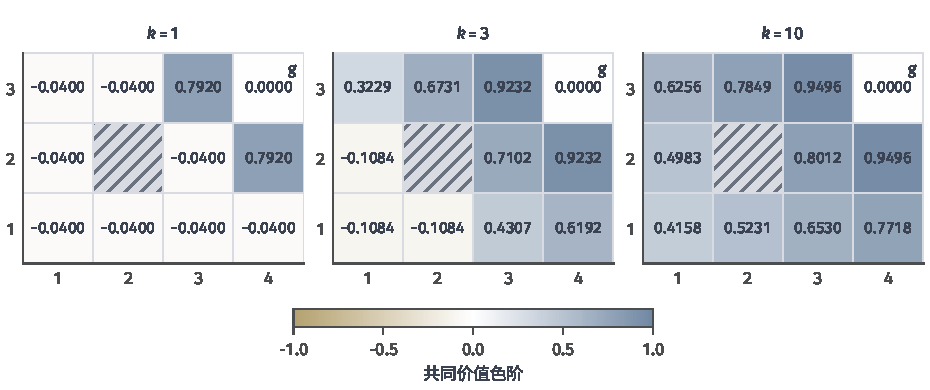
\includegraphics[width=157.400mm]{figures/07-reinforcement-learning/01-problems-and-solving/matplotlib/rl-planning-grid-values.pdf}
 \caption{基准随机网格在$k=1,3,10$次同步价值迭代后的价值，$\gamma=0.9$、$v^{(0)}=0$。数字由完整转移期望计算，显示四位小数；三个面板共用色阶，障碍单独标记。它们是确定的算法迭代值，不是实验学习曲线。}
 \label{fig:rl-planning-grid-values}
\end{figure*}

上述迭代和证书依赖折扣压缩性。若目标只计有限步，我们可以从指定终端值反向算，不需要令迭代趋于无限；若改用平均奖励，累计收益通常不断增长，原价值不动点也不再适用。表~\ref{tab:rl-planning-horizons}~对照这三种任务。平均奖励方程中的差分价值$h(s)$衡量扣除共同增长趋势后的状态差别；表中$T_ah(s)=\sum_{s'}T(s'\mid s,a)h(s')$。对所有状态同时给$h$加同一个常数，方程不变，但存在共同最优平均奖励$g$本身并不保证$h$仅有这种不确定性。例如两个互不连通的零奖励吸收状态都有$g=0$，它们的$h$却可各取任意值；固定其中一个状态的值仍不能确定另一个。参考状态归一化只消除整体常数，唯一性和迭代收敛还须另核结构条件。这些时间目标及其条件可见Puterman的系统论述\scite{rl1-puterman1994-mdp}

表中将用到的通信条件要求：对任意两个状态，都存在某份合法策略，使过程从前一个状态经有限步以正概率到达后一个状态；不同状态对可以使用不同策略。这是在允许选择策略后考察环境中的可达性。固定一份平稳策略后，它诱导的转移链是否不可约，或是否只有一个闭的常返类，则是另一层条件；后一种单链情形还允许暂态状态。通信并不要求每份策略都诱导不可约链，也不能单独保证任意相对价值迭代收敛，表中的迭代条件仍须分别核验。

\begin{table}[htbp]
 \centering
 \small
 \begin{tabularx}{\linewidth}{@{}l>{\raggedright\arraybackslash}X>{\raggedright\arraybackslash}X@{}}
  \toprule
  目标 & 递推与边界 & 关键条件与保证\\
  \midrule
  有限时域 & $V_H=0$，$V_t=\mathcal B_t^*V_{t+1}$；无折扣时取该式$\gamma=1$ & 反向做$H$层；策略一般随$t$变化\\
  无限折扣 & $V^*=\mathcal B^*V^*$ & 有限状态动作、奖励有界、$\gamma<1$；无穷范数压缩\\
  平均奖励 & $g+h(s)=\max_a\{R(s,a)+T_ah(s)\}$ & 需另给通信等条件以得到共同增益$g$；相对价值迭代收敛还需相应非周期或更强混合条件\\
  \bottomrule
 \end{tabularx}
 \caption{不同时间目标的递推口径。平均奖励相对价值迭代通常每轮减去参考状态的备份值来固定$h$的常数，但不能直接套用$\gamma<1$的证明。}
 \label{tab:rl-planning-horizons}
\end{table}

% Outline: 2.2
\section{从动态规划到全局优化}
\label{sec:rl-planning-linear-programming}

刚才的动态规划是逐状态备份、靠反复迭代收敛到最优价值。同一个有限折扣MDP还可以换一个角度：把所有状态动作“最终应满足的关系”一次性写成一组并行的约束，再交给一个优化器统一求解。未知量有两种自然选择：可以是各状态的价值，也可以是策略在折扣时间内分配给各状态动作的访问量。前者给出的约束限制了长期回报的上界，后者的约束则限定哪些访问分布真的能由某份策略实现。下面先分别建立这两个线性规划，再说明它们恰好构成一对互为对偶、最优值相同的问题。

% Outline: 2.2.1
\subsection{价值的线性规划}
\label{sec:rl-planning-value-lp}

最优Bellman方程说明：在状态$s$先取任意合法动作，再最优行动，回报都不能超过$V^*(s)$。我们据此要求候选函数$v$满足
$v(s)\geq R(s,a)+\gamma\sum_{s'}T(s'\mid s,a)v(s')$，对每个状态动作都成立。下一项证明将说明这些约束使$v$成为$V^*$的逐状态上界。既然上界可以任意抬高，我们应将它压低，而不是最大化它。用非负权重$w(s)$指定各状态在目标中的分量，目标和约束都关于$v$线性，得到线性规划（linear programming, LP）：
\begin{equation}
 \begin{aligned}
 \min_v\quad &\sum_s w(s)v(s)\\
 \text{满足}\quad
 &v(s)-\gamma\sum_{s'}T(s'\mid s,a)v(s')\geq R(s,a),
 \quad s\in S,\ a\in\mathsf A(s).
 \end{aligned}
 \label{eq:rl-planning-value-lp}
\end{equation}
式~\eqref{eq:rl-planning-value-lp}~在所有满足Bellman不等式的状态函数中，最小化加权价值。这里的$\min$寻找最紧的上界，并非把策略的回报改成最小化。每个合法动作都对应一条约束；若事先删除某个动作，其长期后果就不再受到检查，可能改变所求上界。

\begin{theorem}[价值线性规划的解]
 \label{thm:rl-planning-value-lp}
 设状态动作有限、动作集非空、奖励有界、$0\leq\gamma<1$的时间齐次MDP，权重$w(s)\geq0$。任意满足每个合法状态动作的Bellman不等式$v(s)\geq R(s,a)+\gamma\sum_{s'}T(s'\mid s,a)v(s')$的$v:S\to\mathbb R$，均逐状态满足$v\geq V^*$。若所有$w(s)>0$，则式~\eqref{eq:rl-planning-value-lp}的唯一最优解为$V^*$。
\end{theorem}
\begin{proof}
 因为每个动作的备份都不超过$v$，这些约束等价于$v\geq \mathcal B^*v$。利用单调性反复备份，
 $v\geq \mathcal B^*v\geq(\mathcal B^*)^2v\geq\cdots$，而压缩性使后者收敛到$V^*$，所以$v\geq V^*$。$V^*$自身满足全部约束，因而可行。对任何不同于$V^*$的可行$v$，至少一个坐标严格大于$V^*$，其他坐标不小于；所有权重严格为正便推出
 $\sum_s w(s)v(s)>\sum_s w(s)V^*(s)$。这同时证明最优性和唯一性。
\end{proof}

若只比较从$\mu_0$出发的回报，可以取$w=\mu_0$；所有约束仍然保留，但零权重状态未必得到唯一价值。例如在走廊之外增加不可达的孤立状态$z$，其唯一动作是零奖励自循环，约束只要求$v(z)\geq\gamma v(z)$，也就是$v(z)\geq0$。当$\mu_0(z)=0$时，任何这样的$v(z)$都不影响目标，而真正的$V^*(z)$为0。因此初始分布下目标已最优，仍不能推出每个坐标都等于全状态最优价值。

% Outline: 2.2.2
\subsection{占用度量的线性规划}
\label{sec:rl-planning-occupancy-lp}

换用访问量作变量时，最需要保证的是：所选的这组概率质量必须真的能由环境中的某份策略产生，而不能脱离动力学任意指派。先回顾第~\ref{chap:rl-overview}~章定义的归一化占用度量
\[
 d^\pi(s,a)=(1-\gamma)\sum_{t=0}^{\infty}
 \gamma^t\mathbb P_\pi(s_t=s,a_t=a),\qquad
 d^\pi(s)=\sum_a d^\pi(s,a).
\]
其中$d^\pi(s)$汇总折扣时间内落在$s$的概率质量。它一部分来自初始分布，另一部分由此前状态动作转移而来。拆出$t=0$项，再对其余时刻使用全概率公式，便得到这种流守恒关系：
\begin{equation}
 \begin{aligned}
 d^\pi(s)
 &=(1-\gamma)\mu_0(s)
   +(1-\gamma)\sum_{t=1}^{\infty}\gamma^t
     \sum_{x,a}\mathbb P_\pi(s_{t-1}=x,a_{t-1}=a)T(s\mid x,a)\\
 &=(1-\gamma)\mu_0(s)+\gamma\sum_{x,a}T(s\mid x,a)d^\pi(x,a).
 \end{aligned}
 \label{eq:rl-planning-flow}
\end{equation}
式~\eqref{eq:rl-planning-flow}~要求一个状态分配给各动作的总量，等于初始注入加折扣后的转移流入。图~\ref{fig:rl-planning-occupancy-flow}~把这两项放回三格走廊：注入为$(1-\gamma)\mu_0$，每条转移流还乘$\gamma$。对所有状态求和，并利用转移概率之和为1，可得
$\sum_{s,a}d^\pi(s,a)=1$。终点吸收后仍占用折扣时间，只是不再产生奖励。

\begin{figure}[htbp]
 \centering
 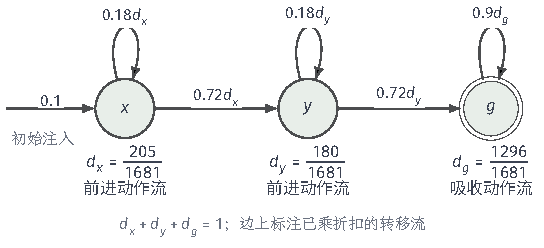
\includegraphics[width=92.050mm]{figures/07-reinforcement-learning/01-problems-and-solving/tikz/rl-planning-occupancy-flow.pdf}
 \caption{手算走廊中前进策略的归一化折扣流。状态流出分别为$d_x,d_y,d_g$；初始注入为$0.1$，前进转移流为$0.72d$，原地流为$0.18d$，终点吸收流为$0.9d_g$。等待动作在最优解中的流量为0，未画出。}
 \label{fig:rl-planning-occupancy-flow}
\end{figure}

这项流约束也会从价值线性规划的对偶中自然出现。取$w=\mu_0$，把每条价值约束写成“右端减左端不大于0”，再引入非负乘子$\lambda(s,a)$。乘子给各约束分配权重，拉格朗日函数把加权约束与原目标相加：
\[
 \begin{aligned}
 L(v,\lambda)
 &=\sum_s\mu_0(s)v(s)
 +\sum_{s,a}\lambda(s,a)[R(s,a)-v(s)]\\
 &\quad+\gamma\sum_{s,a}\lambda(s,a)\sum_xT(x\mid s,a)v(x)\\
 &=\sum_{s,a}\lambda(s,a)R(s,a)+\sum_s v(s)\kappa_\lambda(s),
 \end{aligned}
 \]
将含同一个$v(s)$的项收集后，其系数为
\[
 \kappa_\lambda(s)=\mu_0(s)-\sum_a\lambda(s,a)
       +\gamma\sum_{x,a}T(s\mid x,a)\lambda(x,a).
\]
对固定$\lambda$，取$\inf_v L(v,\lambda)$可为原最小化问题给出下界。由于$v(s)$可以取任意实数，若有一个系数$\kappa_\lambda(s)$非零，就能沿相反方向把$L$降到负无穷；只有全部系数为0才得到有限下界。这个条件正是注入为$\mu_0$的流方程，因而$\lambda$对应总质量为$1/(1-\gamma)$的\emph{未归一化}占用量。对偶在这些可行乘子中最大化下界；代入$d=(1-\gamma)\lambda$，得到
\begin{equation}
 \begin{aligned}
 \max_{d\geq0}\quad&
 \frac{1}{1-\gamma}\sum_{s,a}d(s,a)R(s,a)\\
 \text{满足}\quad&
 \sum_a d(s,a)-\gamma\sum_{x,a}T(s\mid x,a)d(x,a)
   =(1-\gamma)\mu_0(s),\quad s\in S.
 \end{aligned}
 \label{eq:rl-planning-occupancy-lp}
\end{equation}
对偶的$\max$也可以直接理解为：在满足流守恒的访问量中选取累计期望奖励最大的分布。归一化只改变变量尺度，目标仍是$J(\pi)$，所以流注入改为$(1-\gamma)\mu_0$后，目标中的$(1-\gamma)^{-1}$必须保留。接着要验证，这些代数上可行的流确实都对应合法策略。

\begin{theorem}[可行占用量的策略实现]
 \label{thm:rl-planning-occupancy-realization}
 设MDP的状态动作有限、各动作集非空、$0\leq\gamma<1$，初始分布为$\mu_0$。任意非负状态动作函数$d$，若满足对所有$s$的流约束$\sum_a d(s,a)-\gamma\sum_{x,a}T(s\mid x,a)d(x,a)=(1-\gamma)\mu_0(s)$，均可由合法平稳随机策略实现。具体地，令$d(s)=\sum_a d(s,a)$；在$d(s)>0$处取$\pi(a\mid s)=d(s,a)/d(s)$，在$d(s)=0$处任取合法动作分布，则$d=d^\pi$。
\end{theorem}
\begin{proof}
 在正占用状态，按比例选择动作直接给出$d(s,a)=d(s)\pi(a\mid s)$。在零占用状态，各动作量非负且和为0，只能全部为0，因此同一等式仍成立，不依赖该处选什么合法分布。代入流方程，并用列向量$\bm d$收集状态占用量，
 \[
 \bm d=(1-\gamma)\bm\mu_0+\gamma(\bm T^\pi)^\top\bm d.
 \]
 由于$\bm I-\gamma\bm T^\pi$可逆，其转置也可逆，此方程的唯一解为
 \[
 \bm d=(1-\gamma)\sum_{t=0}^{\infty}
 \gamma^t((\bm T^\pi)^\top)^t\bm\mu_0.
 \]
 右端正是策略$\pi$的折扣状态分布。再乘$\pi(a\mid s)$，得到$d(s,a)=d^\pi(s,a)$。零占用状态的任意动作选择没有改变这个唯一解。
\end{proof}

% Outline: 2.2.3
\subsection{价值与占用度量的对偶关系}
\label{sec:rl-planning-duality}

价值线性规划给回报设上界，占用线性规划选取可实现的访问分布；现在需要确认两种求法会不会留下间隙。价值问题可用常数$R_{\max}/(1-\gamma)$作为可行函数，目标又由$V^*$从下方界住。占用问题至少有任意平稳策略的流作为可行点；所有可行$d$非负、总质量为1，且奖励有界，故目标有界。有限维线性规划只要原问题可行且最优值有限，原问题和对偶问题都能达到相同的最优值。这里已核验价值与占用问题的可行性和有界性，因此两种规划的最优目标相等。该强对偶结论及互补松弛的依据可参考\BookChapterRef{chap:optimization}{卷1《数学准备：计算、分析与几何》中讨论最优化的章节}。

我们用示例~\ref{ex:rl-planning-corridor}~检验这种对应。两个非终点处，前进策略的价值都高于等待的一步备份$-0.04+0.9V(s)$，而前进备份恰好等于该价值，因此前进策略满足最优Bellman方程。取$\mu_0(x)=1$，对应流量满足
\[
 d_x=0.1+0.18d_x,\qquad
 d_y=0.72d_x+0.18d_y,\qquad
 d_g=0.72d_y+0.9d_g.
\]
解得
\[
 (d_x,d_y,d_g)=\frac{1}{1681}(205,180,1296).
\]
该策略从不等待，等待动作的流量为0；前进和终点吸收动作分别取得所在状态的全部占用量。将同一组价值与流量代入两个目标，可核对
\[
 \mu_0^\top\bm v^*=V^*(x)=\frac{6718}{8405}
 =10\left(-0.04\frac{205}{1681}
           +0.792\frac{180}{1681}\right).
\]
两个目标确实都等于起点最优价值。终点的占用虽大，却只记录到达后的零奖励时间；它不贡献回报，但不能从归一化流中删除，否则总质量和守恒都将改变。

目标相等还能反推出最优价值上界与最优占用量之间的一个有用刻画。对任意一对可行的$v,d$，Bellman约束的余量非负；将各余量乘对应占用量后求和，再乘归一化还原系数$(1-\gamma)^{-1}$，恰好得到价值目标与占用目标的间隙。若这对解都最优，强对偶使总间隙为零，各项又都非负，因此每个正占用动作对应的约束余量必须为零。这就是下面的互补松弛条件。

这里的余量衡量上界是否紧，不能直接解释为改动作可以获得的收益。例如，只有一个状态和一个动作，奖励恒为0、确定自循环，取$\gamma=1/2$。唯一策略已经最优，其价值为0；可行上界$v=2$却仍有$2-(0+\tfrac12\times2)=1$的余量。此时没有另一个动作可改选，正余量只表明所取价值上界与该策略的占用量没有同时达到最优。下面的定理明确要求$v$与$d$都是相应规划的最优解。

\begin{theorem}[互补松弛与最优动作]
 \label{thm:rl-planning-complementarity}
 设MDP的状态动作有限、各动作集非空、奖励有界、$0\leq\gamma<1$，初始分布为$\mu_0$。$v:S\to\mathbb R$和$d\geq0$分别为式~\eqref{eq:rl-planning-value-lp}（权重$w=\mu_0$）与式~\eqref{eq:rl-planning-occupancy-lp}的最优解。若某合法状态动作满足$d(s,a)>0$，则
 \[
 v(s)=R(s,a)+\gamma\sum_{s'}T(s'\mid s,a)v(s').
 \]
 由$d$按状态归一化恢复的策略在$\mu_0$下最优；仅凭正占用动作的等式，不能断言零占用状态的任意恢复动作也全状态最优。
\end{theorem}
\begin{proof}
 将流约束乘$v(s)$再求和，原始、对偶目标之差恰为
 \[
 \frac{1}{1-\gamma}\sum_{s,a}d(s,a)
 \left[v(s)-R(s,a)-\gamma\sum_{s'}T(s'\mid s,a)v(s')\right].
 \]
 每项由原始与对偶可行性保证非负，强对偶又使总和为0。因此，只要$d(s,a)>0$，对应方括号必须为0，这就是互补松弛。定理~\ref{thm:rl-planning-occupancy-realization}~保证恢复策略实现$d$，其$J$等于对偶目标，故等于$\mu_0^\top\bm v^*$。

 若某状态占用为0，乘积为0就不再限制该处动作的约束余量。例如在不可达孤立状态增加奖励$-1$的自循环动作，选它不会改变从$\mu_0$出发的目标，但其价值为$-1/(1-\gamma)$，低于零奖励自循环。要保证全状态最优，可以在所有状态对真正的$V^*$贪心，或改用严格正的初始权重，求出全状态价值后恢复策略。
\end{proof}

价值变量便于检查各动作的上界，流量变量则便于累计策略的资源消耗。表~\ref{tab:rl-planning-dp-lp}~对照它们与局部备份的检查量。若$c(s,a)$是有界单步成本，只需将占用目标中的奖励换成成本，就能计算该策略的未归一化折扣累计期望：
\[
 \mathbb E_\pi\sum_{t=0}^{\infty}\gamma^t c(s_t,a_t)
 =\frac{1}{1-\gamma}\sum_{s,a}d^\pi(s,a)c(s,a).
\]
所以限制这一成本不超过预算，可以直接增加一条关于$d$的线性约束。这里仅建立计算接口；约束是否可行、是否需要随机化，以及期望成本限制能支持怎样的安全结论，留给第~\ref{chap:rl-trustworthy}~章。

\begin{table}[htbp]
 \centering
 \small
 \begin{tabularx}{\linewidth}{@{}l>{\raggedright\arraybackslash}X>{\raggedright\arraybackslash}X@{}}
  \toprule
  形式 & 求解关系 & 适合检查的量\\
  \midrule
  价值迭代 & 局部Bellman备份 & 全状态残差、贪心损失界\\
  价值LP & 全部动作的上界约束 & 原始可行性、最小上界\\
  占用LP & 非负流及全局守恒 & 对偶间隙；累计成本$\sum dc/(1-\gamma)\leq B$\\
  \bottomrule
 \end{tabularx}
 \caption{递推与全局优化的不同接口。等价的最优目标不意味着通用LP求解器比专用动态规划更快。}
 \label{tab:rl-planning-dp-lp}
\end{table}

% Outline: 2.3
\section{特殊结构下的精确求解}
\label{sec:rl-planning-structure}

前两节按有限MDP的最一般形式求解，代价是每个状态都设一个价值未知量、每个合法动作都要参与比较。当状态数变大时，这套通用方法会很快变得不可承受。但真实问题往往不是“毫无结构的一堆状态和动作”：动力学可能是线性的、成本可能是二次的、最优动作可能随状态有顺序、若干子系统可能彼此独立。如果能识别并利用这些额外关系，就可能不必逐项保存和比较。下面分别考察四类结构，它们依次作用于不同对象：备份能否保持有限参数的价值形式（价值族封闭）、方程能否通过换元变成线性（可线性化）、最优动作能否按状态排序（单调）、以及子问题能否分别求解再合并（可分离）。它们并不是互斥的模型类别，条件成立时可以组合使用。

% Outline: 2.3.1
\subsection{价值函数族的封闭结构}
\label{sec:rl-planning-closure}

在连续状态上逐点保存价值根本无法实现，因为状态有无穷多个取值。一种自然的精确简化是：用有限个参数表示价值，让每次备份只更新这些参数，而不更新一张无限大的表。但这个想法有一个前提必须检查——备份之后的价值仍然属于原来选定的函数族；一旦备份结果跑出了这个函数族，参数更新就无法精确表达它，只能求助近似或扩大表示。\term{Bellman封闭性}（Bellman closure）要求的正是“备份后仍留在所选函数族内”，它使参数化更新能够精确地反复进行。

\begin{definition}[函数族的Bellman封闭性]
 \label{def:rl-planning-closure}
 设$\mathsf V$是状态上的实值函数空间，$\mathcal B:\mathsf V\to\mathsf V$为给定Bellman算子，$\mathcal F\subseteq\mathsf V$。若$\mathcal B\mathcal F\subseteq\mathcal F$，即任意$v\in\mathcal F$经备份后仍属于$\mathcal F$，称$\mathcal F$在$\mathcal B$下封闭。有限时域的相应条件为$\mathcal B_t\mathcal F_{t+1}\subseteq\mathcal F_t$，且指定终端价值属于$\mathcal F_H$。
\end{definition}

仅仅把价值设成参数的线性函数，并不能保证封闭性。考虑连续状态$x$上两个动作，分别给即时奖励$x$和$-x$，随后立即终止。终端零价值属于线性函数族，但一步最优备份是$\max(x,-x)=|x|$，它已经不是$x$的线性函数，备份把函数族“撑破”了。下面的LQR之所以能精确保留二次形式，靠的是线性动力学与二次成本共同提供的特殊结构，而不是任意选一个参数化表示就能做到。

考虑一个状态完全可见的控制系统：一方面希望状态尽量贴近目标（偏离越小越好），另一方面又不希望控制用力过猛。\term{线性二次调节}（linear-quadratic regulation, LQR）恰好分别用线性动力学和二次成本刻画这两点。这里不再使用有限网格，而令状态$\bm x_t\in\mathbb R^{n_x}$、动作$\bm u_t\in\mathbb R^{n_u}$，动作没有额外约束；目标也改为有限时域、无折扣的成本最小化。记从时刻$t$起的最小剩余成本为$C_t$，若把成本取负当作奖励，对应的奖励价值就是$-C_t$。动力学为
\[
 \bm x_{t+1}=\bm A\bm x_t+\bm B\bm u_t+\bm w_t,
 \quad
 \bm A\in\mathbb R^{n_x\times n_x},\
 \bm B\in\mathbb R^{n_x\times n_u}.
\]
加性噪声$\bm w_t$相互独立，并独立于此前状态与动作，均值为0、协方差$\bm\Sigma_t$有限；初始状态固定，或其二阶矩有限。为了在允许的控制序列中比较偏离与用力，我们最小化总期望成本
\begin{equation}
 \mathbb E\!\left[
 \sum_{t=0}^{H-1}
  (\bm x_t^\top\bm Q\bm x_t+\bm u_t^\top\bm R\bm u_t)
 +\bm x_H^\top\bm Q_f\bm x_H\right],
 \label{eq:rl-planning-lqr-cost}
\end{equation}
其中对称矩阵$\bm Q,\bm Q_f\succeq0$分别计入逐步状态成本和终端成本，$\bm R\succ0$计入控制成本；这里$\bm Q$不是动作价值$Q$。反向递推应从指定的终端成本$C_H(\bm x)=\bm x^\top\bm Q_f\bm x$开始，而不默认沿用网格的零终端值。正定的控制成本还将保证每步配方有唯一的最小化动作。

在线性动力学、二次成本、完全可见状态、无额外动作约束和独立零均值加性噪声下，最优剩余成本为$C_t(\bm x)=\bm x^\top\bm S_t\bm x+c_t$，最优动作是线性反馈$\bm u_t^*=-\bm K_t\bm x_t$。矩阵及常数由终端条件反向递推：
\begin{equation}
 \begin{aligned}
 \bm K_t&=(\bm R+\bm B^\top\bm S_{t+1}\bm B)^{-1}
                \bm B^\top\bm S_{t+1}\bm A,\\
 \bm S_t&=\bm Q+\bm A^\top\bm S_{t+1}\bm A
   -\bm A^\top\bm S_{t+1}\bm B
      (\bm R+\bm B^\top\bm S_{t+1}\bm B)^{-1}
      \bm B^\top\bm S_{t+1}\bm A,\\
 c_t&=c_{t+1}+\operatorname{tr}(\bm S_{t+1}\bm\Sigma_t),\\
 \bm S_H&=\bm Q_f,\qquad c_H=0.
 \end{aligned}
 \label{eq:rl-planning-riccati}
\end{equation}
在这组\term{Riccati递推}中，$\bm R+\bm B^\top\bm S_{t+1}\bm B\succ0$，保证每步最小化有唯一动作；$\bm S_t\succeq0$保证下一层仍满足同样条件。噪声二阶矩只进入$c_t$，不改变反馈增益。允许$\bm\Sigma_t$随时刻变化时，每层使用该时刻的协方差即可。有限时域线性二次调节的结论与配方证明可参考\BookChapterRef{chap:control-theory}{卷2《数学准备：概率、因果与决策》中讨论策略的实现与轨迹控制的章节}。

这个结论在规划中的作用是核验Bellman封闭性：终端成本属于“半正定二次型加常数”的函数族，一步最小化后仍在该族内，所以精确规划只需保存矩阵和常数，而不必为每个连续状态存表。若动作改变噪声分布，或决策前必须估计隐藏状态，反馈增益不受噪声影响的结论就不能直接继承。

\begin{example}[标量Riccati递推]
 \label{ex:rl-planning-lqr}
 取教学参数$A=B=Q=R=Q_f=1$、$H=2$。从$S_2=1$得到
 $K_1=1/2$、$S_1=2-1/2=3/2$，再得
 $K_0=(3/2)/(5/2)=3/5$、$S_0=5/2-9/10=8/5$。
 无噪声且$x_0=1$时，$u_0=-3/5$、$x_1=2/5$、
 $u_1=-1/5$、$x_2=1/5$。代入成本，
 \[
 1+\frac{9}{25}+\frac{4}{25}+\frac{1}{25}+\frac{1}{25}
 =\frac85=C_0(1).
 \]
 若两步噪声方差都改为$0.04$，反馈增益不变，
 $c_1=0.04$、$c_0=0.04+1.5\times0.04=0.10$，
 故最优期望成本为$1.70$；这不是同一条确定轨迹的成本。
\end{example}

图~\ref{fig:rl-planning-lqr-closure}~展示这种封闭关系：虽然状态取值无穷，一次精确备份只更新矩阵和常数，执行时再用矩阵乘法计算反馈。一般动作约束可能使配方所得控制不可行，非线性动力学也可能使后继成本不再二次，因而都要重新检查封闭性，不能继续断言价值在整个状态空间上为二次函数。

\begin{figure}[htbp]
 \centering
 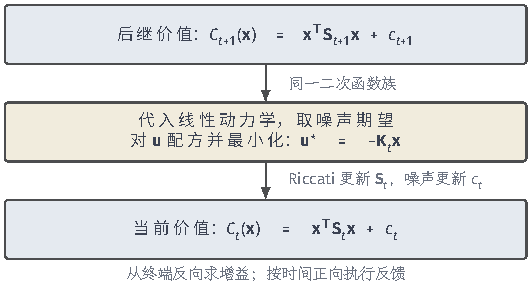
\includegraphics[width=89.958mm]{figures/07-reinforcement-learning/01-problems-and-solving/tikz/rl-planning-lqr-closure.pdf}
 \caption{有限时域LQR的封闭关系。给定线性动力学、二次成本与独立零均值加性噪声，最小化一步成本后仍得到二次价值加常数；增益由反向递推得到，控制按正向时间执行。}
 \label{fig:rl-planning-lqr-closure}
\end{figure}

有限时域封闭还不能保证时域趋于无穷后成本有限。对无噪声、无折扣的无限总成本，标准结果另要求$(\bm A,\bm B)$可稳定、$(\bm Q^{1/2},\bm A)$可检测，并保留$\bm Q\succeq0$、$\bm R\succ0$。可稳定意味着存在反馈，使闭环$\bm A-\bm B\bm K$的特征值落在单位圆内。可检测条件考察成本所衡量的量$\bm Q^{1/2}\bm x$：沿无输入状态动力学始终不能由这个量辨出的状态模式，必须自行衰减，其特征值严格落在单位圆内。这里需要考察模式随时间的演化，不是只检查某个时刻的状态是否满足$\bm Q^{1/2}\bm x=0$；所用的量也不是传感器观测，不能把这项成本条件替换成观测核的性质。在这些条件下，零终端成本的递推随时域延长，收敛到唯一半正定稳定化解$\bm S$。它满足将式~\eqref{eq:rl-planning-riccati}~中的$\bm S_t,\bm S_{t+1}$都替换成$\bm S$所得的代数Riccati方程。

这个无限时域结论还要求稳定化解，而不是任意代数方程解。持续非零噪声通常会使无折扣无限总成本发散，需要改用平均成本等准则；有限时域的常数项可以求出，并不代表无限累加仍有限。

% Outline: 2.3.2
\subsection{价值方程的可线性化结构}
\label{sec:rl-planning-kl-control}

LQR通过保留二次价值族减少了未知量，但每一步仍要做二次函数最小化和矩阵求逆。另一类结构走的是不同的简化路线：它不去限制价值的函数形式，而是限制“能选择哪些后继分布、偏离自然规律要付多少代价”，从而让原本含优化的价值方程可以通过一次换元变成线性方程。考虑这样一种控制视角：直接把下一步状态的概率分布当作可选择的对象；系统在不加干预时本来有一个自然转移，干预越强、分布偏离自然转移越多，费用就越高。\term{KL控制}用KL散度来计量这种偏离。要特别注意，它允许优化的是一族受支持约束的后继分布，而不是普通MDP里事先给定的那几个离散动作。

在普通MDP中，执行动作$a$只能得到接口规定的$T(\cdot\mid s,a)$；即使随机化动作，得到的也只是这些给定分布的凸组合，无法任意调配各后继的概率。KL控制的特殊设定则把“在自然规律已有的可能后继中重新分配概率”本身当作可选控制，并对偏离收费。因此两种接口即便支持的后继集合相同，也不代表物理执行器真能实现任意的概率重分配；使用下面的换元技巧前，必须先确认任务确实赋予了这种控制权限和对应的费用规则。

两个有限分布$p,q$之间的KL散度是按$p$平均的对数概率比：
\[
 D_{\mathrm{KL}}(p\Vert q)=\sum_{i:p_i>0}p_i\log\frac{p_i}{q_i}.
\]
$p_i=0$的项取0；若$p_i>0$而$q_i=0$，值为正无穷。对数取自然底。该量非负，且仅在$p=q$时为0，一般并不对称。只要将待优化成本改写成“一个不随候选改变的常数加非负KL项”，就能验证候选的全局最优性。这些性质以及收益与KL偏离权衡的指数倾斜结论，可参考\BookChapterRef{chap:information-theory-and-statistical-geometry}{卷2《数学准备：概率、因果与决策》的“概率分布的分析与优化”章}。

\begin{definition}[有限时域KL控制]
 \label{def:rl-planning-kl-control}
 给定非空有限状态集$S$、整数时域$H\geq1$、被动转移概率核$T_0(s'\mid s)$、有限实值成本$c_t:S\to\mathbb R$（$0\leq t<H$）和$g:S\to\mathbb R$，以及$\lambda>0$。在状态$s$可选择概率分布$u(\cdot\mid s)$，要求
 $T_0(s'\mid s)=0$时$u(s'\mid s)=0$。单步期望成本为
 \[
 c_t(s)+\lambda D_{\mathrm{KL}}(u(\cdot\mid s)\Vert T_0(\cdot\mid s)).
 \]
 目标是在所有允许的历史依赖分布控制中，最小化从$t$到$H-1$的上述成本之和加$g(s_H)$的期望，不折扣。最小剩余成本记为$V_t^{\mathrm c}(s)$，终端条件为$V_H^{\mathrm c}=g$；对应的奖励价值为$-V_t^{\mathrm c}$。
\end{definition}

被动转移$T_0$表示不施加这种分布控制时的自然规律。支持约束使控制只能重新分配自然规律已有的可能后继，不能以有限费用创造原本概率为零的转移。对支持内概率采用$0\log0=0$约定；严格正的$\lambda$保证偏离确实增加成本，控制必须权衡这项费用与未来成本。

给定下一时刻的最小成本$V_{t+1}^{\mathrm c}$，当前要在允许的概率分布$u$中，最小化KL费用加后继成本期望。我们先用被动概率和后继成本构造一个候选：令
$Z_t(s)=\sum_{s'}T_0(s'\mid s)\exp(-V_{t+1}^{\mathrm c}(s')/\lambda)>0$作为归一化系数，并取
\[
 u_t^*(s'\mid s)=
 \frac{T_0(s'\mid s)\exp(-V_{t+1}^{\mathrm c}(s')/\lambda)}{Z_t(s)}.
\]
有限状态、有限成本及$\lambda>0$保证$Z_t(s)>0$，候选$u_t^*$是合法概率分布，且与$T_0$有相同支持。有限分布的指数倾斜关系在这个支持集上给出：任意允许分布$u$的待优化成本满足
\begin{equation}
 \begin{aligned}
 &\lambda D_{\mathrm{KL}}(u\Vert T_0)
       +\sum_{s'}u(s'\mid s)V_{t+1}^{\mathrm c}(s')\\
 &\qquad=\lambda D_{\mathrm{KL}}(u\Vert u_t^*)-\lambda\log Z_t(s).
 \end{aligned}
 \label{eq:rl-planning-kl-completion}
\end{equation}
右侧第二项不随$u$改变，第一项非负且在$u=u_t^*$时为0。因此$u_t^*$在整个允许分布集合上达到最小值，不只满足一阶必要条件。加回当前状态成本，得到
\[
 V_t^{\mathrm c}(s)=c_t(s)-\lambda\log Z_t(s).
\]
这个最小值替代了原来的分布优化。$u_t^*$给低成本后继更大的指数权重，再由$T_0$和$Z_t$保持支持与归一化；指数中的负号来自成本越小越优，不能原样解释为奖励最大化中的偏好。

上式仍含对数，但我们可以改求成本的指数变换，而不直接求成本。令$z_t(s)=\exp(-V_t^{\mathrm c}(s)/\lambda)$，对等式两侧取相应指数，便有
\begin{equation}
 z_t(s)=\exp(-c_t(s)/\lambda)\sum_{s'}T_0(s'\mid s)z_{t+1}(s'),
 \qquad z_H(s)=\exp(-g(s)/\lambda).
 \label{eq:rl-planning-kl-linear}
\end{equation}
后继未知量$z_{t+1}$现在只出现在加权和中，所以这是线性反向递推。由终端值算出$z$后，再用
$u_t^*(s'\mid s)=T_0(s'\mid s)z_{t+1}(s')/\sum_xT_0(x\mid s)z_{t+1}(x)$
恢复最优转移，若需成本则用$V_t^{\mathrm c}=-\lambda\log z_t$还原。控制限制、指数变换和不同时间目标的关系可参见Todorov的原始工作\scite{rl2-todorov2006-linear}

用一个只剩一步的教学模型检查这种权衡。被动转移以相等概率到达两处，终端成本分别为0和$\lambda\log3$，当前状态成本为0。两处$z_H$为1和$1/3$，所以$Z=2/3$，最优受控概率为$(3/4,1/4)$，最小成本为$\lambda\log(3/2)$。若全部转向第一处，终端成本虽为0，偏离被动分布的费用却为$\lambda\log2$，总成本更高。因此最优分布仍给第二个后继保留概率。

线性化依赖刚才的控制费用和时间目标。表~\ref{tab:rl-planning-kl-regimes}~对照有限时域、终止型和平均成本中的边界条件。一般折扣成本方程含$\gamma V(s')$，同样换元得到$z(s)=e^{-c(s)/\lambda}\sum_{s'}T_0(s'\mid s)z(s')^\gamma$，通常仍然非线性。即使方程已经线性，也未必减少未知量个数：表格表示仍需保存每个状态的$z(s)$。

终止型总成本把固定时刻的终端边界改成首次到达终点集$B$时终止，并在到达状态支付给定成本$g_B$。这一行采用不随时间变化的状态成本$c(s)$，令$N=S\setminus B$为非终点集合。将被动核$T_0$按这两个集合分块，$\bm T_{NN}$收集从$N$到$N$的概率，$\bm T_{NB}$收集从$N$到$B$的概率，行均对应出发状态。对角矩阵$\bm G_N=\operatorname{diag}_{s\in N}(e^{-c(s)/\lambda})$给出非终点的成本因子，边值$\bm z_B=e^{-\bm g_B/\lambda}$按坐标取指数，因而方程中只剩$\bm z_N$未知。这是按状态集合分块，不是有限时域递推中的时间下标；表中的谱半径条件保证这组线性方程唯一可解，有限最优总成本还须另核终止问题的适定条件。

\begin{table*}[htbp]
 \centering
 \small
 \begin{tabularx}{\linewidth}{@{}l>{\raggedright\arraybackslash}X>{\raggedright\arraybackslash}X@{}}
  \toprule
  目标 & 换元后的关系 & 所需边界或附加条件\\
  \midrule
  有限时域 & $\bm z_t=\bm G_t\bm T_0\bm z_{t+1}$ & $\bm G_t=\operatorname{diag}(e^{-c_t/\lambda})$，终端$\bm z_H=e^{-\bm g/\lambda}$\\
  终止型总成本 & $\bm z_N=\bm G_N(\bm T_{NN}\bm z_N+\bm T_{NB}\bm z_B)$ & 固定终点集$B$的边值；如$\bm G_N\bm T_{NN}$的谱半径小于1，线性方程唯一可解\\
  平均成本 & $e^{-\bar c/\lambda}\bm z=\bm G\bm T_0\bm z$ & 有限不可约被动链、有限成本给正的Perron特征向量；只确定尺度，非周期性影响幂迭代\\
  一般折扣成本 & $\bm z=\bm G\bm T_0\bm z^\gamma$ & 幂按坐标作用；不再是线性方程\\
  \bottomrule
 \end{tabularx}
 \caption{KL控制的三类线性形式及折扣边界。终止型的$N$表示非终点集合，不是时间；平均成本的$\bar c$是每步最优平均成本。}
 \label{tab:rl-planning-kl-regimes}
\end{table*}

表中的平均成本关系来自$\bar c+V^{\mathrm c}(s)=c(s)-\lambda\log\sum_{s'}T_0(s'\mid s)e^{-V^{\mathrm c}(s')/\lambda}$的指数变换。此时$V^{\mathrm c}$是扣除平均增长后的差分成本，换元所得$z$只确定到尺度。不可约非负矩阵的Perron理论保证所需正特征向量；沿轨迹累加成本等式，再除以时长，有界差分成本的首尾项消失，从而验证平均成本最优性。这条证明使用特征值与平均成本关系，不是折扣压缩论证。

% Outline: 2.3.3
\subsection{最优策略的单调与阈值结构}
\label{sec:rl-planning-monotone}

在库存这类问题中，状态（库存数量）和动作（订货多少）本身都是可以排序的。如果每个库存水平都单独与所有动作逐一比较，就忽略了最优选择可能天然带有顺序规律。不过在使用顺序结构前，必须先说清动作究竟代表什么：当库存增加时，“订货量”可能下降，但“订货之后的总库存”却可能上升，两者的单调方向相反。\term{单调策略}指状态沿一个方向增大时，所选动作也始终沿某个固定方向变化；对只有两个动作的情形，这种规则往往只由一个切换点决定，称为\term{阈值策略}。库存中的\term{基库存策略}以$x$表示订货前的净库存，把订后库存设为$\max\{x,S_t\}$，订货量为$(S_t-x)_+$；其中$(z)_+=\max(z,0)$表示正部，所以库存一旦达到水平$S_t$就不再订货。这类规则把要描述的选择压缩成少数几个阈值或水平，但$S_t$具体取多少仍须根据模型和目标求出来。

怎样判断这种顺序关系是否真的成立？关键在于比较“选大动作比选小动作多花多少成本”如何随状态变化。如果状态越大，大动作相对小动作反而越便宜，那么最优选择就应当随状态增大而单调地偏向大动作。把当前成本与后继成本期望合起来记作一步目标$f(s,a)$，称它具有\term{递减差分}，若对$s_2\geq s_1$、$a_2\geq a_1$，
\begin{equation}
 f(s_2,a_2)-f(s_2,a_1)
 \leq f(s_1,a_2)-f(s_1,a_1).
 \label{eq:rl-planning-decreasing-differences}
\end{equation}
这个条件比较的是两动作成本之差，而不是要求每个动作的绝对成本下降。以下定理在共同的有限全序动作集中最小化$f$；遇到并列最小值时，统一选最大的动作，才能得到所述单调选择。更一般的格上比较静态结果见Topkis\scite{rl2-topkis1978-lattice}

\begin{theorem}[递减差分给出单调最优动作]
 \label{thm:rl-planning-monotone}
 设$(S,\leq)$为全序状态集，所有状态共享同一个非空有限全序动作集$\mathsf A$，$f:S\times\mathsf A\to\mathbb R$为一步成本目标。若对任意$s_2\geq s_1$、$a_2\geq a_1$都有$f(s_2,a_2)-f(s_2,a_1)\leq f(s_1,a_2)-f(s_1,a_1)$，则选取最大的最小化动作
 $a^*(s)=\max\arg\min_a f(s,a)$得到随$s$单调不减的策略。
\end{theorem}
\begin{proof}
 取$s_2\geq s_1$，记$a_1=a^*(s_1)$、$a_2=a^*(s_2)$。反设$a_2<a_1$。最优性给出
 $f(s_1,a_1)-f(s_1,a_2)\leq0$与
 $f(s_2,a_1)-f(s_2,a_2)\geq0$。递减差分又给出
 \[
 0\leq f(s_2,a_1)-f(s_2,a_2)
 \leq f(s_1,a_1)-f(s_1,a_2)\leq0.
 \]
 所有不等式只能取等号，故$a_1$也是$s_2$处的最小化动作。但$a_1>a_2$，与$a_2$是最大的最小化动作矛盾。因此$a_2\geq a_1$。
\end{proof}

将定理用于多步决策，还必须证明后继成本加入后，差分条件仍保持。考虑一个可逐步验证的排队模型：状态$x\in\{0,\ldots,B\}$表示有容量上限的队长，动作$a=0$保留队列，$a=1$立即清空。保留支付非负且随$x$不减的等待成本$h(x)$，清空支付固定成本$K>0$。随后产生与状态动作独立、分布已知的非负到达$W_t$，容量外到达丢弃且不另收费。两动作的后继分别为
$\min(x+W_t,B)$和$\min(W_t,B)$。取有限时域、无折扣、终端成本0。

若$C_{t+1}$单调不减，则
\[
 \begin{aligned}
 f_t(x,0)&=h(x)+\mathbb E C_{t+1}(\min(x+W_t,B)),\\
 f_t(x,1)&=K+\mathbb E C_{t+1}(\min(W_t,B)).
 \end{aligned}
 \]
保留目标随$x$不减，清空目标不随$x$变化，取两者最小值得到的$C_t$仍随$x$不减。从$C_H=0$反向归纳，这项性质逐步保持。与此同时，清空相对保留的成本差$f_t(x,1)-f_t(x,0)$随$x$不增，满足递减差分。因此在上述模型中，可以按阈值选择清空。若清空费用依赖队长、丢包另有复杂成本，或到达规律随服务动作变化，就必须重新验证每一步目标，不能只凭“排队模型”沿用阈值结论。

为求出阈值而不只说明其存在，取教学参数$B=5$、$h(x)=x$、$K=2.5$、$W_t=1$、$H=2$。最后一步最小成本为$C_1(x)=\min(x,2.5)$。在$t=0$，清空目标恒为$2.5+C_1(1)=3.5$，保留目标为$x+C_1(\min(x+1,5))$；后者在$x=0,1,2$分别为1、3、4.5，且继续随$x$不减。因此从$x=2$起清空更便宜，阈值为2，见图~\ref{fig:rl-planning-threshold}。

\begin{figure}[htbp]
 \centering
 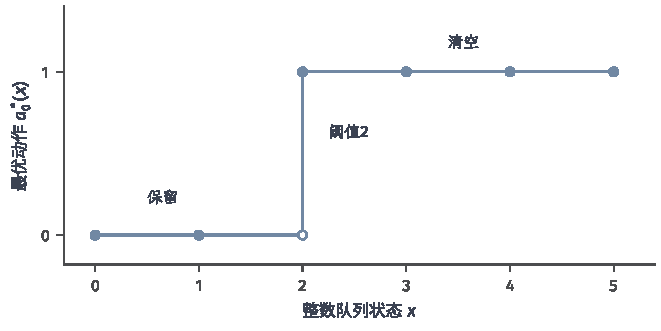
\includegraphics[width=112.000mm]{figures/07-reinforcement-learning/01-problems-and-solving/matplotlib/rl-planning-threshold.pdf}
 \caption{上述两步排队教学模型在$t=0$的最优动作。横轴是整数队长，纵轴0表示保留、1表示清空；连接线只帮助阅读阶梯形状，不表示连续状态模型。阈值2由列出的Bellman目标计算。}
 \label{fig:rl-planning-threshold}
\end{figure}

回到库存时，订后库存$y$受$y\geq x$约束，各状态的允许动作不同，不能直接套用共同动作集的定理。采用有限时域、无折扣的经典教学模型：净库存$x,y$取实数，负值表示结转的欠货；订货立即到达，无容量上限，也不允许通过负订货量处置库存。各期非负需求$D_t$分布已知、独立于过去和订货选择，需求后净库存为$y-D_t$。没有固定订货费，单位费$c\geq0$；以有限凸函数$\ell_t(z)$表示需求后净库存$z$的持有和缺货成本，以有限凸函数$C_H$表示终端成本。一步目标于是为
\[
 \begin{aligned}
 C_t(x)&=\min_{y\geq x}\{c(y-x)+
       \mathbb E[\ell_t(y-D_t)+C_{t+1}(y-D_t)]\}\\
       &=-cx+\min_{y\geq x}G_t(y),\\
 G_t(y)&=cy+\mathbb E[\ell_t(y-D_t)+C_{t+1}(y-D_t)].
 \end{aligned}
\]
还要求所列期望在每个实数$y$处有限，并且每期$G_t$在\emph{整个实数域}有有限的全局最小化点$S_t$；例如$G_t(y)\to+\infty$当$|y|\to\infty$，就是保证最小点存在的充分条件。仅要求每个$y\geq x$的受限问题能取到最小值并不够：若需求、持有和缺货成本及终端成本全为0而$c>0$，则$G_t(y)=cy$在每个受限域都于$x$取最小，却没有全域有限最小点。

若$C_{t+1}$凸，平移后的$\ell_t(y-D_t)+C_{t+1}(y-D_t)$对$y$仍凸，取期望保持凸性，再加线性项$cy$，得到凸的$G_t$。$-cx+G_t(y)$对$(x,y)$联合凸，约束$y\geq x$也为凸集合：两状态与各自最优订后库存的凸组合仍可行，把它代入目标便得到$C_t$的凸性不等式。因此从$C_H$反向归纳，凸性逐期保持。任取上述全局最小点$S_t$，当$x\leq S_t$时它可行且最优；当$x>S_t$时，凸函数在$S_t$右侧单调不减，受限最小值于$x$取到。故可选$y^*=\max(x,S_t)$，并非要求最优动作唯一。

例如最后一期取确定需求$D_{H-1}=2$、$c=1$、$\ell_{H-1}(z)=(z)_++3(-z)_+$、$C_H=0$，则$G_{H-1}(y)$在$y\leq2$时为$6-2y$，在$y\geq2$时为$2y-2$，从而$S_{H-1}=2$。订前库存1时订1，库存3时不订；订后库存随$x$不减，订货量随$x$不增。加入固定订货费、容量限制等条件后，目标或可行域改变，策略形状须重新推导。

% Outline: 2.3.4
\subsection{整体价值与策略的可分离结构}
\label{sec:rl-planning-separable}

当系统由若干彼此独立的设备组成时，联合状态是各设备状态的笛卡尔积，规模会随设备数急剧膨胀。我们很自然地希望分别求出每个子设备的局部价值、再相加，而不去枚举全部联合状态。但能否这样做，不只取决于各设备是否独立转移、奖励是否可加，还取决于动作选择是否也能各自独立进行：如果几台设备共享同一个操作者、每一步只能操作其中一台，就无法在同一时刻同时选取各自的最优动作。下面先给出直接分解成立所需的条件，再用反例说明共享资源会破坏其中的哪一步。

\begin{theorem}[独立子过程的可分离性]
 \label{thm:rl-planning-separable}
 设$m\geq1$个子过程具有有限状态集$S_i$、非空有限动作集$\mathsf A_i(s_i)$、转移核$T_i$及有界奖励$R_i$，共同折扣因子为$0\leq\gamma<1$。联合状态为$s=(s_1,\ldots,s_m)\in\prod_i S_i$，合法联合动作集是$\mathsf A(s)=\prod_i\mathsf A_i(s_i)$，且
 \[
 T(s'\mid s,a)=\prod_iT_i(s_i'\mid s_i,a_i),\qquad
 R(s,a)=\sum_iR_i(s_i,a_i).
 \]
 在有限状态动作的折扣问题中，$V^*(s)=\sum_iV_i^*(s_i)$，且各子过程的最优动作可分别选择。有限时域中，若各时刻仍满足上述乘积转移与可加奖励，终端价值也可加，则相同的价值分解及逐分量动作选择按时刻成立。
\end{theorem}
\begin{proof}
 对任意可加函数$v(s)=\sum_i v_i(s_i)$，利用转移的乘积形式并对其他坐标求和，
 \[
 \sum_{s'}T(s'\mid s,a)v(s')
 =\sum_i\sum_{s_i'}T_i(s_i'\mid s_i,a_i)v_i(s_i').
 \]
 因为每个$a_i$可以独立地在$\mathsf A_i(s_i)$中选择，
 \[
 \begin{aligned}
 (\mathcal B^*v)(s)
 &=\max_{a_1,\ldots,a_m}\sum_i
   \left[R_i(s_i,a_i)+\gamma\sum_{s_i'}T_i(s_i'\mid s_i,a_i)v_i(s_i')\right]\\
 &=\sum_i(\mathcal B_i^*v_i)(s_i).
 \end{aligned}
 \]
 最后一个等式的两个方向分别来自“任意动作的和不超过各自最大值之和”和“同时选择每个最大化动作便达到该和”。有限时域由可加终端值反向归纳，且逐层的独立最大化恢复策略。折扣情形取各子过程不动点$v_i=V_i^*$，其和成为联合$\mathcal B^*$的不动点；唯一性给出联合最优价值，独立最大化动作构成联合最优策略。
\end{proof}

图~\ref{fig:rl-planning-factorization}~上部的两个子网格各自接收动作，允许同时执行局部最大化选择；若改为每步最多激活一个，证明中把联合最大值拆成各自最大值之和的等式就不再成立。一个最小反例是两个单状态设备：激活每步得1，空闲得0，状态恒定。在笛卡尔积动作下可同时激活，联合价值为$2/(1-\gamma)$；互斥激活后只能得到$1/(1-\gamma)$。因此独立转移不足以保证局部最优价值相加。

\begin{figure}[htbp]
 \centering
 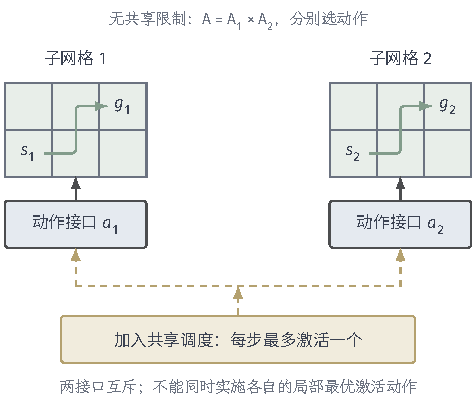
\includegraphics[width=80.617mm]{figures/07-reinforcement-learning/01-problems-and-solving/tikz/rl-planning-factorization.pdf}
 \caption{可分解的动力学不等于可分解的决策。上部两个子网格分别接收$a_1,a_2$；下部共享调度选择只能激活一个接口，使联合动作集不再是原局部动作集的笛卡尔积。}
 \label{fig:rl-planning-factorization}
\end{figure}

共享激活虽然破坏了直接相加，但若结构足够特殊，仍可能找到避免联合枚举的办法。\term{经典冻结型Markov老虎机}（rested Markov bandit）把每个独立设备看成一只“臂”：只有当前被激活的那只臂才会发生状态转移并产生奖励，其余臂的状态一律冻结、奖励为0；每步恰好激活一只臂，且切换不收费。若每只臂只有一个不变状态，问题就简化为每步从若干奖励来源中选一个；现在每只臂内部还会随激活演化，所以当前选择也会影响以后可得的奖励。在有限状态、已知转移、有界非负奖励、共同$0<\gamma<1$及无限时域目标下，Gittins指数定理给出一个结构性结论：可以给每只臂在当前状态下单独算出一个数（指数），然后每一步只需激活当前指数最大的那只臂，无须维护联合状态上的价值表。奖励规律未知、必须边试验边估计的老虎机探索，则由第~\ref{chap:rl-learning}~章讨论。

这个数要衡量的不是“下一步奖励”，而是“持续使用这只臂一段时间，平均每单位折扣时间能换来多少收益”，从而允许为了将来的高收益先承受眼前的低收益。对臂$i$当前状态$x$，我们允许根据已看到的局部历史决定何时停止，且至少激活一次；在所有这样的停止规则中，取期望累计奖励与期望累计折扣时间之比的上确界：
\begin{equation}
 \nu_i(x)=\sup_{\tau\geq1}
 \frac{\mathbb E_x\sum_{t=0}^{\tau-1}\gamma^t R_i(X_t)}
      {\mathbb E_x\sum_{t=0}^{\tau-1}\gamma^t},
 \label{eq:rl-planning-gittins}
\end{equation}
其中$X_t$是持续激活该臂时的局部状态过程，$\tau$是由该臂已见历史决定的停止时刻，$\tau\geq1$保证分母为正。固定一份停止规则并反复运行时，先分别计算收益与折扣占用时间的期望，再将两者相除；这通常不同于先算每条轨迹的收益时间比再取平均。允许在看到不利局部状态后停止，正是它区别于当前一步奖励的地方。用上确界容纳所有允许的停止规则，不要求某个有限停止时刻必定取到它。也可以把候选指数$\lambda$当作每次激活的机会成本，考察净收益
$\sup_{\tau\geq1}\mathbb E_x\sum_{t<\tau}\gamma^t(R_i(X_t)-\lambda)$，
净收益由正转为非正的临界$\lambda$给出上述指数。全局最优性并非来自价值直接相加，而是利用未激活臂的冻结性，交换比较竞争臂的激活片段，证明按指数排序不损失回报。完整指数理论与局部计算方法见Gittins的原文\scite{rl2-gittins1979-index}

用一个两状态教学例观察指数为何不同于即时奖励。某臂从$x$开始，激活时奖励为0并确定转到$y$；在$y$激活时奖励为1，且状态保持$y$。未激活时两状态都冻结，奖励为0，取$\gamma=1/2$。若连续激活$k\geq1$次后停止，时间按该臂的激活次数计算，这条确定轨迹的收益与折扣占用时间之比为
\[
 \frac{\sum_{t=1}^{k-1}2^{-t}}{\sum_{t=0}^{k-1}2^{-t}}
 =\frac{2^{k-1}-1}{2^k-1}
 =\frac12-\frac{1}{2(2^k-1)}.
\]
激活一次的比率为0，激活两次为$1/3$，随$k$增加趋于$1/2$。由于状态演化确定，非随机停止规则在这条轨迹上就是选择停止次数；随机停止也不能超过这些比率的上确界，因为每条轨迹的收益都至多为其折扣占用时间的一半，分别取期望后该不等式仍成立。因此$\nu_i(x)=1/2$，虽然$x$的即时奖励为0。只允许有限停止时，没有某个有限$k$取到这一上确界；若允许永久激活，则得到同一数值。这个例子展示了继续激活的未来收益怎样进入指数，全局指数规则的最优性仍依赖前述冻结性等条件。

若未激活的臂也会演化，即restless情形，等待期间的状态会改变，刚才利用冻结性交换片段的依据就不再适用；任意有限截止日期或切换成本也不在此定理范围内。各臂内部仍可能具有封闭、可线性化或单调结构，但简化局部计算并不自动解决共享激活造成的全局耦合。

% Outline: 2.4
\section{有限预算下的当前状态规划}
\label{sec:rl-planning-local-search}

前面的精确方法都是在行动之前，就为整个状态空间算出价值或反馈律。但很多实时系统做不到这一点：导航机器人此刻就需要下一步动作，没有预算先把成千上万甚至无穷多个状态全部算完。于是出现另一条思路——只为“当前所在的这一个状态”向前展开可能发生的后果，据此立刻给出一个动作；等真正走到新状态后，再在那里重新展开一次。这称为局部搜索。它把计算时间集中花在当前决策上，代价是不保存覆盖全部状态的完整解，因此每次到达新状态往往都要重新搜索。

% Outline: 2.4.1
\subsection{有限预算下的近似规划问题}
\label{sec:rl-planning-local-budget}

设机器人已经位于某个网格状态，当前这次规划只需返回一个动作，也可以附带给出各候选动作的价值估计。评价这样一个规划器要同时看两件事：首动作的长期后果是否选得好，以及它是否赶在行动截止时间之前算出来、用了多少次模型查询、占用多少搜索内存。这里要特别区分两种预算：全状态方法可能先花较长时间离线预计算，但执行时只需查一次表；局部方法几乎不需要预计算、总查询量也可能更少，但单次搜索仍可能超时。因此比较二者时，预计算预算和行动时预算应分别记账。

图~\ref{fig:rl-planning-search-tree}~展示了一次局部搜索可以从四个方面控制规模：限制向前看的步数（深度）、限制每层展开的分支数（宽度）、在停止展开处补上对未来价值的估计（叶值）、以及根据已有结果决定下一次模拟走哪条路径（自适应分配）。它们裁剪的是同一棵树的不同部分，可以组合使用；后文将分别分析每种手段省下了什么计算、又留下了什么误差。

\begin{figure}[htbp]
 \centering
 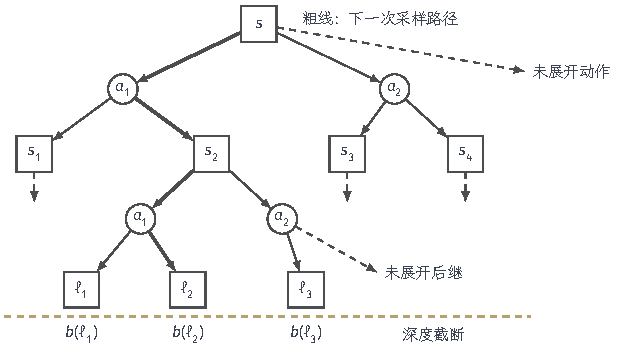
\includegraphics[width=105.138mm]{figures/07-reinforcement-learning/01-problems-and-solving/tikz/rl-planning-search-tree.pdf}
 \caption{局部搜索中的四种预算安排。方框是状态处的动作选择，圆点是选定动作后的随机后继选择；虚线边表示未展开的分支，底部虚线表示深度截断，叶子处的$b$为剩余价值估计。加粗路径表示下一次模拟的一个可能样本路径，不表示确定的环境转移。}
 \label{fig:rl-planning-search-tree}
\end{figure}

具体怎样展开，仍由模型接口决定：若模型直接给出非零概率的后继，就可以逐个列出并加权求精确和；若只有生成模型，一次查询只产生一个随机后继，就必须靠重复查询的均值来估计期望。无论哪种接口，都要严格区分树中的两类节点——哪些是规划器可以选择的动作，哪些是动作之后只能接受、无法挑选的随机结果。规划器能决定“查询哪个动作”，却不能在看到随机后继后专挑最有利的那个当作必然结果；即使采样完全正确，有限次模拟仍会带来统计误差。

% Outline: 2.4.2
\subsection{未来步数受限的搜索空间构造}
\label{sec:rl-planning-horizon-search}

一棵无限向前生长的搜索树在计算上不可行，最直接的裁剪是只看有限步：先精确计算当前状态$s$起$H$步内的奖励，至于第$H$步之后那部分尚未展开的未来，则用一个边界函数$b$给出估值补上。允许策略$\sigma$在这$H$步内根据实际到达的状态选择合法动作，以期望折扣回报最大为准，在这些策略中取上确界：
\begin{equation}
 U_H^b(s)=\sup_\sigma\mathbb E_\sigma\!\left[
 \sum_{t=0}^{H-1}\gamma^t r_t+\gamma^H b(s_H)
 \,\middle|\,s_0=s\right].
 \label{eq:rl-planning-lookahead}
\end{equation}
这里$b(s_H)$是到达搜索边界时对剩余回报的估计，它要乘$\gamma^H$，是因为这部分回报从第$H$步才开始计算，折算回当前时刻必须整体打$H$次折扣。式中的策略$\sigma$能够根据实际观察到的后继随时调整后续动作，因此我们优化的是一棵“看到结果再决定下一步”的反馈决策树，而不是一条事先定死、无法回应随机滑移的动作序列。在有限状态动作下，可以从$U_0^b=b$出发，逐层用$U_h^b=\mathcal B^*U_{h-1}^b$精确算出这棵树。特别要注意，取$b=0$只是在计算时忽略搜索范围之外的回报，相当于一种近似，并没有真的把任务改成在第$H$步终止——真实的终点奖励可能仍在更远处。

\term{滚动时域规划}（receding-horizon planning）的用法是：每次求出这棵有限树后只执行根部的第一个动作；待观察到实际新状态，再从那里重新规划同样长度的$H$步。这样能根据真实滑移不断修正后续选择，但“重新规划”本身并不会自动补回边界之外被忽略的价值。要判断有限前瞻究竟有多准，仍须控制边界估值的误差、以及它如何随层数向根部传播。

\begin{theorem}[有限前瞻的终端误差]
 \label{thm:rl-planning-terminal-error}
 设时间齐次MDP的状态动作有限、各动作集非空、奖励满足$|r_t|\leq R_{\max}<\infty$，且$0\leq\gamma<1$。给定整数$H\geq1$和终端函数$b,\tilde b:S\to\mathbb R$，$U_H^b$表示从当前状态起在所有合法反馈策略中最大化前$H$步折扣奖励加$\gamma^H b(s_H)$所得的价值。则
 \[
 \lVert U_H^b-U_H^{\tilde b}\rVert_\infty
 \leq\gamma^H\lVert b-\tilde b\rVert_\infty.
 \]
 特别地，若$\lVert b-V^*\rVert_\infty\leq\varepsilon$，
 则$\lVert U_H^b-V^*\rVert_\infty\leq\gamma^H\varepsilon$；
 零终端值满足
 $\lVert U_H^0-V^*\rVert_\infty\leq\gamma^H R_{\max}/(1-\gamma)$。
 固定同一策略序列、比较其两个终端估值时，同样成立。
\end{theorem}
\begin{proof}
 对任意同一策略序列，两个$H$步目标的前$H$步奖励相消，差只剩
 $\gamma^H\mathbb E[b(s_H)-\tilde b(s_H)]$，绝对值不超过
 $\gamma^H\lVert b-\tilde b\rVert_\infty$。对两个目标分别取上确界，利用
 $|\sup f-\sup g|\leq\sup|f-g|$，该界仍成立。也可逐层使用期望的非扩张性和最大化的非扩张性，每层再乘$\gamma$，得到同一结果。

 取$\tilde b=V^*$时，$\mathcal B^*V^*=V^*$保证$U_H^{V^*}=V^*$，即得第二条。又因$\lVert V^*\rVert_\infty\leq R_{\max}/(1-\gamma)$，令$b=0$得到零边值界。它也等于直接控制尾和
 $\sum_{t=H}^{\infty}\gamma^t|r_t|\leq\gamma^H R_{\max}/(1-\gamma)$所得的界。
\end{proof}

终端误差界控制的是$H$步前瞻值，还不是滚动执行策略的价值。若每次使用相同$H$、边界函数$b$及固定并列规则，精确根动作便定义一个平稳策略。计算根动作时，当前奖励后面接的是剩余$H-1$步的$U_{H-1}^b$，所以该策略对$U_{H-1}^b$贪心，不是对$U_H^b$贪心。由定理~\ref{thm:rl-planning-greedy-loss}，当$H\geq1$且$\lVert b-V^*\rVert_\infty\leq\varepsilon$时，其长期损失至多
$2\gamma^H\varepsilon/(1-\gamma)$。这才把前瞻精度与反复执行的性能联系起来。

\begin{example}[同一障碍下的短前瞻]
 \label{ex:rl-planning-detour}
 为隔离时域的影响，采用基准网格的坐标、障碍和终点，但将起点改为$(1,2)$，取消滑移，使合法动作确定执行；奖励和$\gamma=0.9$不变，所有搜索使用$b=0$。从起点向上绕过障碍，最短4步到终点；向下进入底部通道，至少6步到终点。

 长度$L$的确定到达路径的回报为
 $-0.04\sum_{t=0}^{L-2}0.9^t+0.9^{L-1}$。
 当$H=2$时，上、下动作的最优截断回报都为$-0.076$，按“下优先”的并列规则会选下。当$H=4$时，向上的分支已经看到终点，回报为$0.6206$；向下的分支仍只有四次步成本，回报为$-0.13756$。完整6步底部路线的回报为$0.426686$，也低于上方路线。
\end{example}

图~\ref{fig:rl-planning-detour}~让我们看到，短前瞻的并列来自两条分支都还没有计入终点收益。重复短规划未必解决这个问题：始终取$H=1$和“下、上、右、左”的并列次序，起点会向下，底部左格又向上，形成往返。若某个早期动作不可逆，后来即使延长搜索，也不能撤销已经付出的损失。

\begin{figure}[htbp]
 \centering
 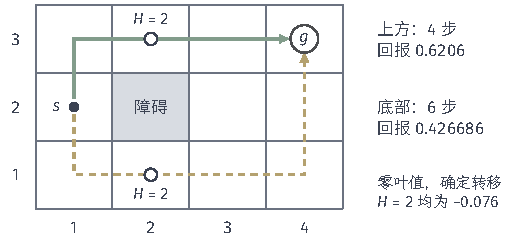
\includegraphics[width=86.847mm]{figures/07-reinforcement-learning/01-problems-and-solving/tikz/rl-planning-detour.pdf}
 \caption{确定性教学变体中的两条绕行路线。实线为4步上方路线，虚线为6步底部路线；标记$H=2$说明两个首动作在零叶值下都尚未看到终点。图中条件仅用于示例~\ref{ex:rl-planning-detour}，不替代基准随机网格。}
 \label{fig:rl-planning-detour}
\end{figure}

% Outline: 2.4.3
\subsection{未来分支受限的搜索空间构造}
\label{sec:rl-planning-sparse-search}

即使把深度限制为$H$，这棵树仍然可能太宽：每个状态都有若干候选动作，每个动作之后又有若干随机后继。裁剪宽度有两种性质完全不同的做法，必须分清：限制动作数是在删掉规划器本来可以选择的选项，可能因此漏掉真正最优的动作；限制随机后继数则不改变可选动作，只是用有限样本来近似“执行该动作后期望发生什么”。后者保留了动作选择本身，却引入了采样误差。

\term{稀疏采样}（sparse sampling）采取后一种做法：保留对有限动作的逐一枚举，但只为每个动作从生成模型独立抽取$m$个后继，再递归地计算这些样本上的未来价值，用样本均值近似随机后果的期望。取零叶值时，递归写为
\begin{equation}
 \begin{aligned}
 \widehat U_0(s)&=0,\\
 \widehat Q_h(s,a)&=\frac1m\sum_{j=1}^{m}
       \bigl[r_j+\gamma\widehat U_{h-1}^{(j)}(s'_j)\bigr],\\
 \widehat U_h(s)&=\max_{a\in\mathsf A(s)}\widehat Q_h(s,a).
 \end{aligned}
 \label{eq:rl-planning-sparse-sampling}
\end{equation}
其中$j$编号的是同一$(s,a)$下的样本$(r_j,s'_j)$，不是轨迹时刻；$\widehat U_{h-1}^{(j)}$来自第$j$棵递归子树，而非同一张表的第$j$轮更新。每棵子树继续使用新样本。若每处动作数至多为$A$，一层为$A$个动作各付出$m$次查询，并为每个样本建立子树，因此
$C_0=0$、$C_h\leq Am(1+C_{h-1})$，进而
$C_H\leq\sum_{\ell=1}^{H}(Am)^\ell$。计数不显含全状态数，却仍可能随深度迅速增长。

我们还要判断这些有限样本能否可靠选择根动作。若$R_{\max}=0$，奖励、零叶值递推的理想值和采样估计都恒为0，估计误差也恒为0，无须使用尾概率界。下面只在$V_{\max}>0$时分析波动。先保留理想子值$U_h^0$，只分析一次均值估计；有界奖励和折扣使
$r+\gamma U_{h-1}^0(s')\in[-V_{\max},V_{\max}]$。
对一个动作的$m$个独立样本，Hoeffding不等式给出：$m$个独立、同分布于$[-V_{\max},V_{\max}]$内的随机变量，其均值偏离期望超过$\eta>0$的概率至多$2\exp[-m\eta^2/(2V_{\max}^2)]$。该界用于为每个模型查询均值分配允许的失败概率；独立有界随机量的集中条件可参考\BookChapterRef{chap:random-sequences-and-processes}{卷2《数学准备：概率、因果与决策》的“随机序列与随机过程”章}。
树中需要估计的动作均值至多有
$M=A\sum_{\ell=0}^{H-1}(Am)^\ell$个。即使节点状态由祖先样本决定，在给定祖先后，该节点的新样本仍独立，且相同的概率界一致成立。因此联合失败概率至多
$2M\exp[-m\eta^2/(2V_{\max}^2)]$。

只控制根部的一次均值还不够，实际计算使用的是带误差的递归子值。为了分开抽样波动与子树误差，对剩余$h$层的一个节点和动作，先用同一批$(r_j,s'_j)$配合理想子值，构造辅助均值
\[
 \widetilde Q_h(s,a)=\frac1m\sum_{j=1}^{m}
       [r_j+\gamma U_{h-1}^0(s'_j)].
\]
它的期望是理想动作价值
$Q_h^0(s,a)=R(s,a)+\gamma\sum_{s'}T(s'\mid s,a)U_{h-1}^0(s')$。
前面的集中界控制的是$|\widetilde Q_h-Q_h^0|$；实际估计$\widehat Q_h$与辅助均值的差，则只来自同一批后继处使用了不同的子值。在树内所有辅助均值误差均不超过$\eta$的联合事件上，令$e_{h-1}$同时界住相关子树的估值误差，三角不等式给出
\[
 \begin{aligned}
 |\widehat Q_h(s,a)-Q_h^0(s,a)|
 &\leq |\widehat Q_h(s,a)-\widetilde Q_h(s,a)|
       +|\widetilde Q_h(s,a)-Q_h^0(s,a)|\\
 &\leq\gamma e_{h-1}+\eta.
 \end{aligned}
\]
对合法动作取最大值不会放大这个统一误差上界，因而剩余$h$层的状态估值误差满足
$e_h\leq\eta+\gamma e_{h-1}$、$e_0=0$，从而
$e_H\leq\eta(1-\gamma^H)/(1-\gamma)$。
根部各动作值的误差也有同样上界；按估计值选动作相对理想$H$步最优首动作的损失不超过$2e_H$。再单独加上截断误差，才能联系无限时域目标。选择$m$使上述失败概率不超过指定$\alpha$便得到一条充分保证；$M$也依赖$m$，故这是需满足的隐式条件，而不是忽略树大小的一次均值估计。

上述保证依赖独立生成查询、有限动作、奖励界，以及对整棵有限树的误差联合控制，不能只靠某个节点的均值准确。Kearns等给出了更系统的分析：当前状态规划可以不显含全状态数，但精度要求和有效时域，即折扣尾部尚不能忽略的步数，仍可能使查询代价很高\scite{rl2-kearns2002-sparse}

固定$m$会为各节点预先分配相同宽度，也可以把展开数量与实际访问次数联系起来。\term{渐进加宽}（progressive widening）在节点访问少时保留少量候选，随着访问增加再加入动作或后继。图~\ref{fig:rl-planning-widening}~对照同一个父节点的预设宽度与增长宽度；这改变的是展开预算，不会自动提供最优性保证。

\begin{figure}[htbp]
 \centering
 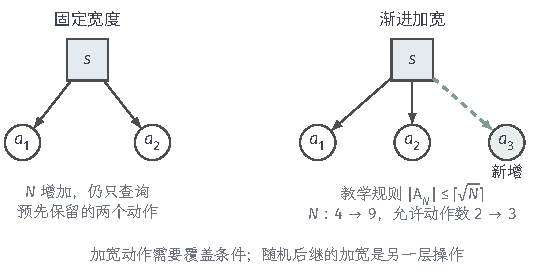
\includegraphics[width=90.318mm]{figures/07-reinforcement-learning/01-problems-and-solving/tikz/rl-planning-widening.pdf}
 \caption{固定分支与渐进加宽。左侧预先只保留两个动作；右侧在节点访问次数$N$增加后加入第三个动作，虚线标记本次新增边。若加宽的是随机后继而非动作，应在每个动作节点内部另行实施，不能混为同一次动作筛选。}
 \label{fig:rl-planning-widening}
\end{figure}

例如以节点访问次数$N$限制动作数为$\lceil cN^\beta\rceil$，其中$c>0$、$0<\beta<1$，使候选数增长慢于访问数，给已有候选留下重复评估的预算。在连续动作中，还要说明怎样提出新动作、最优动作附近能否被采到，以及邻近动作价值是否足够接近。若加宽随机后继，保留与重采样也必须保持正确的转移概率含义。这些条件缺失时，树变大仍不构成最优性证书。

% Outline: 2.4.4
\subsection{搜索空间外的未来价值评估}
\label{sec:rl-planning-leaf-value}

当搜索在一个尚未到达终点的格子停止展开时，后续奖励仍然真实存在、仍属于任务目标，只是我们没有继续把树画下去。因此需要对“这部分未展开的回报”给出一个估值，作为式~\eqref{eq:rl-planning-lookahead}~中的边界函数$b$，这就是\term{边界价值评估}。常见的有四种来源，它们补在搜索树的同一个边界位置，但所评价的后续行为和代价各不相同：直接取零等于忽略它；启发式依据问题知识估一个数；基础策略的\term{rollout}从叶子出发按某条既定规则继续模拟、再累计所得奖励；近似价值函数则用一组共享参数直接对叶子求值。

固定示例~\ref{ex:rl-planning-detour}~中的两处叶子$p=(2,3)$和$q=(3,2)$，它们在确定性变体中都恰好距终点两步。最佳剩余回报同为$-0.04+0.9=0.86$。表~\ref{tab:rl-planning-leaf-values}~在这同一对叶子上比较四种接口；所有数字均为教学设定。

\begin{table*}[htbp]
 \centering
 \small
 \begin{tabularx}{\linewidth}{@{}lcc>{\raggedright\arraybackslash}X>{\raggedright\arraybackslash}X@{}}
  \toprule
  边界规则 & $b(p)$ & $b(q)$ & 额外调用 & 偏差与方差\\
  \midrule
  零值 & $0$ & $0$ & 0 & 忽略真实剩余回报，无采样方差\\
  距离启发式 & $0.9$ & $0.9$ & 已知距离时为0 & 只计终点折扣、漏计步成本；此例高估$0.04$\\
  基础策略rollout & $0.86$ & $0.6206$ & 每条轨迹分别2、4次 & 基础策略在$q$多走两步；确定性模型中方差为0\\
  近似价值函数 & $0.80$ & $0.82$ & 求值时为0 & 给定的教学预测；相对$V^*$误差分别$-0.06,-0.04$\\
  \bottomrule
 \end{tabularx}
 \caption{固定叶子的四类评估。rollout基础策略在$p$走$p\to(3,3)\to g$，在$q$走$q\to(3,1)\to(4,1)\to(4,2)\to g$；预测数值不是训练实验结果，计算或训练这些预测的前期代价未计入在线调用。}
 \label{tab:rl-planning-leaf-values}
\end{table*}

表中的rollout差别来自基础策略的路线，而不是采样波动。模型随机时，rollout估计的仍是所选基础策略$\pi_{\mathrm b}$的$V^{\pi_{\mathrm b}}$，不自动是$V^*$。平均$N$条独立完整回报可减小采样方差，却不会改变基础策略的次优性。若只模拟$L$步再置零，还会相对$V^{\pi_{\mathrm b}}$留下至多$\gamma^L V_{\max}$的尾误差。折扣任务可能没有自然终止，因此完整rollout也未必能在有限次调用内结束。

定理~\ref{thm:rl-planning-terminal-error}~给出了资源取舍：减小边界误差或增加深度，都能降低传到根部的误差上界。加深会扩大搜索树，改进叶值则可能复用之前算出的价值。不过，网络在其他区域预测准确，不能代替当前搜索叶子上的误差控制。这里先讨论如何使用叶值；跨状态表示和评价近似价值的方法由下一节展开。

% Outline: 2.4.5
\subsection{搜索预算的自适应分配}
\label{sec:rl-planning-mcts}

如果在同一个根状态反复模拟，很快会出现一个资源分配问题：有些动作已经模拟很多次、证据较充分，有些动作几乎没试过、价值仍很不确定。若每次都对所有分支平均用力，往往不划算。\term{蒙特卡罗树搜索}（Monte Carlo tree search, MCTS）的思路是保存各节点的访问统计，用已有的模拟结果决定下一次该往哪条路径深入：一次模拟从根出发，沿已建成的树选择动作，遇到尚未充分展开的节点就扩展，再评估叶子的回报，最后把沿途奖励连同折扣后的叶值逐层回传、更新统计。整个过程中要分清两种选择：树内“走哪条分支继续模拟”由搜索规则决定，而动作之后到达哪个后继仍由模型随机采样，二者不能混为一谈。

这些统计量按搜索树节点分别保存。同一个环境状态可能由不同路径到达，也可能对应不同的剩余深度；它在树中的这些节点各有自己的访问次数和平均回报。下面的$N(s,a)$、$\bar Q(s,a)$用节点所处的环境状态$s$作简记，省略路径与剩余深度标记，不表示仅按环境状态共享统计。若另做节点合并，至少须保留剩余深度，并核对后续模型、合法动作与叶值规则是否相同；仅凭环境状态相同不足以合并这些统计量。

为了同时利用“已知回报较高的动作”和“还没怎么试过的动作”，在当前节点的每条动作边$(s,a)$上记录访问次数$N(s,a)$和从该边起算的平均折扣回报$\bar Q(s,a)$，并令$N(s)=\sum_aN(s,a)$。\term{UCT}（upper confidence bounds applied to trees）给每个动作打一个由两部分相加的分数，用它决定树内下一次模拟走哪条边；对已访问的合法动作，选择分数最大的一个：
\begin{equation}
 a\in\arg\max_a\left[
 \bar Q(s,a)+c\sqrt{\frac{\log N(s)}{N(s,a)}}\right],
 \label{eq:rl-planning-uct}
\end{equation}
第一项$\bar Q$是“利用”：偏向目前平均回报高的动作；第二项随$N(s,a)$增大而减小，是“探索”：访问得越少的动作，这项加分越大，越有机会补充证据。其中$c>0$要与回报的数值尺度相配；未访问过的动作先至少试一次，以免分母为零。要强调的是，这个分数只用于决定把查询预算投向哪里，第二项并不是环境真正给出的奖励。预算用尽、需要输出最终动作时，通常按访问次数或平均回报来选、不再加探索项，因此报告时必须写明最终采用的规则。

图~\ref{fig:rl-planning-mcts}~用一条教学记录展示分数、叶值和回传怎样共同改变预算。人为给定根状态$(1,1)$两条边的统计量：
$N(\text{右})=4,\bar Q(\text{右})=0.30$，
$N(\text{上})=1,\bar Q(\text{上})=0.20$，
取$c=0.20$。UCT分数分别约为$0.427$与$0.454$，因此下一次模拟先试“上”。假定本次没有滑移，到达$(1,2)$，当步奖励$-0.04$，叶估值$b=0.70$；回传值为
$g=-0.04+0.9\times0.70=0.59$。
这是假设的单次搜索记录，$0.70$不是该状态的真实最优价值。更新后
$N(\text{上})=2$，
$\bar Q(\text{上})=(1\times0.20+0.59)/2=0.395$。
此时两条分数约为$0.434$与$0.584$，下一次仍偏向“上”。一次乐观叶估值会改变后续预算，因此访问次数大并不自行证明估值正确。

\begin{figure}[htbp]
 \centering
 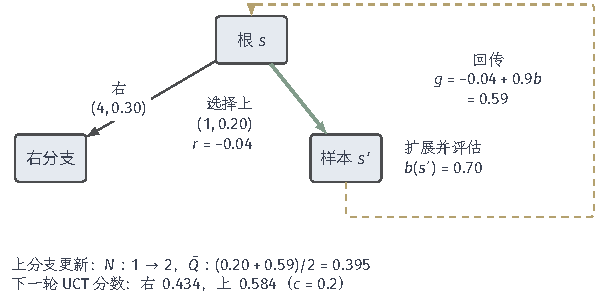
\includegraphics[width=101.388mm]{figures/07-reinforcement-learning/01-problems-and-solving/tikz/rl-planning-mcts.pdf}
 \caption{一次MCTS模拟及回传。边标签列出模拟前的$(N,\bar Q)$；本次选择“上”，扩展到样本后继，用$b=0.70$评估叶子，并回传$0.59$，得到更新后的$(2,0.395)$。箭头旁分别标明树内选择与统计量回传，数字为正文规定的教学记录。}
 \label{fig:rl-planning-mcts}
\end{figure}

若路径更深，先从叶值开始，用$g_t=r_t+\gamma g_{t+1}$逐层算回各边起点的回报，再更新对应边的统计量：
$N\leftarrow N+1$、
$\bar Q\leftarrow\bar Q+(g_t-\bar Q)/N$。
各边的奖励起算时刻和折扣次数不同，因此不能把根部累计回报原样写入所有深度。

UCT的探索项借鉴了老虎机的上置信界（upper confidence bound, UCB），即给证据不足的动作增加乐观估值。不过，树内下游搜索规则会不断改变，同一边以后模拟的回报分布未必与早期相同，不能直接套用固定分布老虎机的全部结论。原始UCT分析在有限动作、有界回报和有限深度等条件下沿树深归纳，处理这种变化；折扣问题还需加入截断误差。即使原设定下一致，也不代表任意先验、叶网络或连续加宽方案都有相同有限样本保证\scite{rl2-kocsis2006-uct}

在棋类中，合法走子和状态转移由规则给定，难点是无法穷举全部后续局面。AlphaZero把网络给出的动作先验和局面价值接入搜索：先验提示哪些动作先分配预算，价值估计尚未展开的未来，模型仍由已知规则提供。因此学习这些建议不等于学习环境动力学\scite{rl2-silver2018-alphazero}

具体地，AlphaZero使用带策略先验的PUCT式选择，按先验概率调整探索分配，其典型探索项与
$p(a\mid s)\sqrt{N(s)}/(1+N(s,a))$成正比，而非直接照抄式~\eqref{eq:rl-planning-uct}。表~\ref{tab:rl-planning-alphazero}~区分环境规则、动作先验、叶值与搜索统计的职责。

\begin{table*}[t]
 \centering
 \small
 \begin{tabularx}{\linewidth}{@{}l>{\raggedright\arraybackslash}X>{\raggedright\arraybackslash}X@{}}
  \toprule
  部件 & 无学习先验的基本搜索 & AlphaZero中的接口\\
  \midrule
  环境后果 & 用精确规则或模型样本展开 & 已知棋类规则，不以学习动力学为必要条件\\
  动作预算 & 根据均值和探索项分配 & 策略先验影响早期访问分配；先验错误可能浪费预算\\
  叶子价值 & 零值、启发式或rollout & 价值网络估计当前局面结果，仍有逼近误差\\
  搜索输出 & 根动作及其统计量 & 根访问分布提供动作选择依据，并作为策略训练目标\\
  训练反馈 & 可以完全没有训练阶段 & 自我对弈结果训练价值；对手策略与自我对弈训练记录的分布随策略变化\\
  \bottomrule
 \end{tabularx}
 \caption{已知模型搜索中规则、先验、叶值和搜索目标的不同作用。棋类回报与双方轮流行动的符号按当前玩家处理，不能直接套用单智能体网格的同向回报。}
 \label{tab:rl-planning-alphazero}
\end{table*}

已知规则、动作建议和叶值承担不同职责，搜索可以组合给定转移规则、动作先验与叶节点价值。先验与价值如何从自我对弈中改进、对手策略和自我对弈训练记录的分布怎样随之变化，则涉及多个决策者的共同学习，由第~\ref{chap:rl-multi-agent}~章继续分析。

% Outline: 2.5
\section{面向全状态的近似规划}
\label{sec:rl-planning-global-approximation}

局部搜索每次到达新状态都要重新展开，若导航过程中反复经过同一位置或相似局面，这些计算彼此无法复用，会造成大量重复。另一条近似路线针对这一点：保存一个覆盖全部状态的价值函数，但用数目有限的、跨状态共享的参数来表示它，代替为每个状态单独存一个数。这样能同时降低存储和重复计算，却引入了新问题——更新一个参数会同时改变许多状态的预测。本节就要分析这种“共享”如何影响价值评价和动作选择，以及在什么误差范围内结果仍然可用。

% Outline: 2.5.1
\subsection{全状态规划的挑战}
\label{sec:rl-planning-global-budget}

基准网格的11个合法位置可以各存一个价值。但只要状态再包含若干离散变量，表格就会迅速膨胀：如果导航还要考虑$q$种物品的库存、每种有$L$个取值，状态数就从单纯的位置扩大为位置与库存组合，共有$11L^q$个。取教学规模$L=10,q=6$，已有约1100万个状态；每值占8字节，仅价值表就要约8800万字节。再加入时间、动作或设备台数，存储和转移表还会继续暴涨。更关键的是，即使“库存如何变化”的规则本身只有短短几行，状态组合的数量也不会因此减少——规则简洁不等于组合可以低成本枚举。

价值表示被压缩后，一次规划更新内部其实包含好几类不同的计算，误差来源也各不相同。图~\ref{fig:rl-planning-approximation-loop}~把它们分开：表示决定哪些状态共享参数，Bellman备份计算转移期望，拟合用选定的函数类去近似备份目标，动作选择再做最大化。相应地至少要分清四种误差：表示或拟合误差（函数类能否表达目标）、期望估计误差（用样本代替精确求和）、以及动作优化误差（数值求解有没有真正取到最大值），不能把它们笼统称为一个“预测误差”。

\begin{figure*}[htbp]
 \centering
 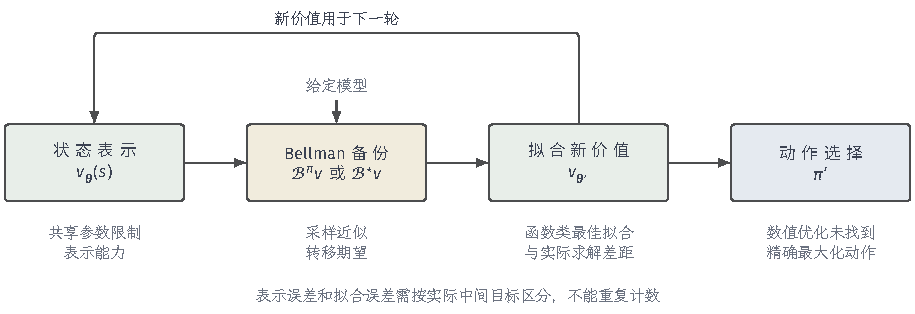
\includegraphics[width=154.961mm]{figures/07-reinforcement-learning/01-problems-and-solving/tikz/rl-planning-approximation-loop.pdf}
 \caption{全状态近似的共同计算接口。实线表示当前价值、备份目标、拟合结果与动作选择之间的计算依赖，外侧回路表示把新价值送往下一轮；下方分别标出表示、期望估计、拟合和动作优化可能产生的误差。给定模型仍是备份的输入。}
 \label{fig:rl-planning-approximation-loop}
\end{figure*}

这些计算仍以给定模型为输入。为了减少精确求和而使用模型样本，会留下有限样本的期望估计误差；模型本身若由真实交互学得，还会偏离环境规律，那是下一章要加入的另一层误差。本节只分析给定模型上的表示和求解，不把两种误差混称为来源不明的预测误差。

% Outline: 2.5.2
\subsection{跨状态近似价值的表示}
\label{sec:rl-planning-representation}

要用少数参数代替庞大的价值表，最直接的办法是让一整组状态共用同一个数值。\term{状态聚合}（state aggregation）就是这样一种分组表示：取一个映射$g:S\to\{1,\ldots,p\}$，令$v(s)=\theta_{g(s)}$，于是更新参数$\theta_i$会同时改变第$i$组所有状态的预测。分组的关键在于把“长期回报确实相近”的状态放在一起，而不能只凭几何上相邻就归为同组，否则被迫共享的误差会很大。

比硬分组更细的是\term{基函数展开}：让状态通过一组给定特征以加权和的形式贡献价值。用$\bm\phi(s)\in\mathbb R^p$表示特征向量、$\bm\theta$表示权重，写成
$\ v_{\bm\theta}(s)=\bm\phi(s)^\top\bm\theta$。
例如在网格中取$\bm\phi(s)=(1,x/4,y/3)^\top$，就只需保存3个参数便能为任意位置求值；代价是这样只能表示坐标的仿射函数，既不能任意指定11个格子的价值，也不会自动刻画“必须绕过障碍”这种非线性结构。若把特征取成各组的指示函数，基函数展开就退化为状态聚合。更一般的参数化函数（如神经网络）还能表达非线性关系，但它能表示哪些函数仍取决于网络结构和参数数量。

图~\ref{fig:rl-planning-aggregation}~用同一网格检查分组会丢失什么。按行聚合把障碍两侧的$(1,2)$和$(3,2)$放在同组，但两处最优价值约为$0.501527$和$0.801271$。共享常数不可能同时等于它们，最大误差至少为差值的一半，约$0.149872$。按到达终点的通道划组能够保留两侧差别，却没有证明组内所有价值相同；还须继续检查组内误差。

\begin{figure}[htbp]
 \centering
 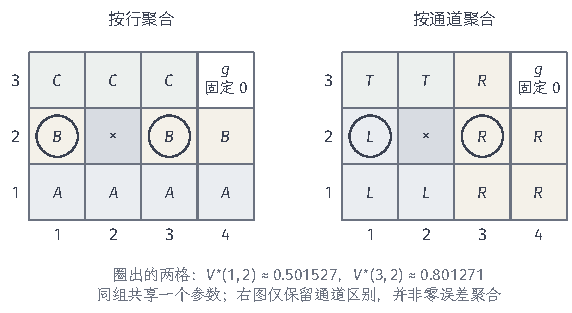
\includegraphics[width=96.788mm]{figures/07-reinforcement-learning/01-problems-and-solving/tikz/rl-planning-aggregation.pdf}
 \caption{同一基准网格的两种教学聚合。左图按行分成A、B、C组，右图按障碍周围的通道分成L、T、R组；非终点格的字母表示共享参数，终点价值固定为0，颜色仅作辅助。右图保留了障碍两侧的区别，但不是精确MDP同态或零误差聚合的声明。}
 \label{fig:rl-planning-aggregation}
\end{figure}

表~\ref{tab:rl-planning-representations}~分别比较一次价值求值与一次单状态参数更新所需的资源，其中$n_S=|S|$表示状态数。更灵活的函数类可能减小表示偏差，但投影迭代未必更稳定，数值优化也未必能找到最佳拟合。

\begin{table*}[htbp]
 \centering
 \small
 \begin{tabularx}{\linewidth}{@{}lcc>{\raggedright\arraybackslash}X@{}}
  \toprule
  表示 & 参数存储 & 求值／单样本更新 & 表达范围与限制\\
  \midrule
  全状态表 & $O(n_S)$ & $O(1)$／$O(1)$ & 可独立表示每个状态，不含模型存储\\
  $p$组聚合 & $O(p)$ & $O(1)$／$O(1)$ & 假设组索引可常数时间取得；组内差别全部丢失\\
  $p$维稠密线性特征 & $O(p)$ & $O(p)$／$O(p)$ & 只能表示特征张成空间；未计特征构造和批量解方程\\
  一般参数化函数 & 参数数$p_\theta$ & 依计算图而定 & 前向与反向代价须按架构计数；非凸拟合与泛化另需分析\\
  \bottomrule
 \end{tabularx}
 \caption{价值表示的资源口径。一次函数求值不包括Bellman备份所需的多后继求值；动作价值$q(s,a)$若为每个动作单独输出，还需计入动作维。}
 \label{tab:rl-planning-representations}
\end{table*}

% Outline: 2.5.3
\subsection{策略的近似价值评估}
\label{sec:rl-planning-approximate-evaluation}

固定策略$\pi$和线性函数空间$\mathcal F$后，目标是在这个有限表示里尽量逼近它的真实价值$V^\pi$。这里出现一个现实困难：如果真实价值$V^\pi$已知，直接拿状态—真实价值对$(s,V^\pi(s))$作回归即可，但规划时未知的恰恰就是$V^\pi$；我们真正拿得到的，只是由模型确定的Bellman关系。因此需要区分几种“在不知道$V^\pi$时仍可计算”的近似目标。为比较它们，先固定状态权重$\xi(s)>0$、$\sum_s\xi(s)=1$，以
$\lVert v\rVert_\xi^2=\sum_s\xi(s)v(s)^2$计量加权平方大小。优化在$\mathcal F$中寻找对应误差最小的函数；投影则把一次备份的结果变成该加权距离下最接近的可表示函数。

\begin{definition}[三种近似评价对象]
 \label{def:rl-planning-projected-evaluation}
 给定状态动作有限、奖励有界且$0\leq\gamma<1$的时间齐次MDP，$\pi$为合法平稳策略，$V^\pi$为其折扣价值。设$\mathcal F\subseteq\mathbb R^{|S|}$是线性子空间，$\xi(s)>0$且$\sum_s\xi(s)=1$，$\Pi_\xi$为加权内积$\langle u,v\rangle_\xi=\sum_s\xi(s)u(s)v(s)$下到$\mathcal F$的正交投影。三种近似评价问题分别为
 \[
 \begin{array}{ll}
 \text{价值拟合：}&\displaystyle\min_{v\in\mathcal F}\lVert v-V^\pi\rVert_\xi^2,\\
 \text{残差最小化：}&\displaystyle\min_{v\in\mathcal F}\lVert v-\mathcal B^\pi v\rVert_\xi^2,\\
 \text{投影方程：}&v=\Pi_\xi \mathcal B^\pi v,\qquad v\in\mathcal F.
 \end{array}
 \]
 前两者最小化不同误差；第三者要求一次备份后投影回来不再改变$v$，并不要求原始Bellman残差为零。
\end{definition}

定义中的价值拟合直接缩小预测与$V^\pi$的差，残差最小化缩小预测与自身备份的差；投影方程则寻找备份再投影后的不动点。因此后两者不要求先取得各状态的真实价值$V^\pi(s)$作为拟合目标，也不保证给出第一种答案。在线性表示中，我们可以将投影方程化为关于参数的线性系统：用$\bm\Phi\in\mathbb R^{n_S\times p}$的第$s$行为$\bm\phi(s)^\top$，
$\bm D=\operatorname{diag}(\xi)$，并假设$\bm\Phi$列满秩。投影矩阵为
$\bm\Pi_\xi=\bm\Phi(\bm\Phi^\top\bm D\bm\Phi)^{-1}\bm\Phi^\top\bm D$。
将$\bm v=\bm\Phi\bm\theta$代入投影方程并乘$\bm\Phi^\top\bm D$，得到
\begin{equation}
 \underbrace{\bm\Phi^\top\bm D(\bm I-\gamma\bm T^\pi)\bm\Phi}_{\bm A}
 \bm\theta
 =\underbrace{\bm\Phi^\top\bm D\bm r^\pi}_{\bm b}.
 \label{eq:rl-planning-projected-system}
\end{equation}
式~\eqref{eq:rl-planning-projected-system}~把函数不变条件压缩成$p$个参数的方程。但$\bm\Phi$列满秩只保证投影矩阵中的逆存在，不自动保证这里的$\bm A$可逆。只有后者可逆，$\bm A^{-1}\bm b$才是唯一参数解；若奇异，还需检查有无解、怎样选解，或是否另加正则化。正则化是改变方程的求解选择，不是原方程无条件可解的证明。

\begin{example}[同一特征的三种答案]
 \label{ex:rl-planning-projection}
 构造一个独立的两状态、单动作教学模型，$\gamma=1/2$，
 \[
 \bm T^\pi=\begin{pmatrix}0&1\\0&1\end{pmatrix},\quad
 \bm r^\pi=\begin{pmatrix}1\\0\end{pmatrix},\quad
 \bm\Phi=\begin{pmatrix}1\\2\end{pmatrix},\quad
 \bm D=\tfrac12\bm I.
 \]
 精确价值为$(1,0)^\top$。价值拟合最小化
 $\tfrac12[(\theta-1)^2+4\theta^2]$，故$\theta=1/5$。
 原始残差为$(1+\theta,\theta)^\top-(\theta,2\theta)^\top=(1,-\theta)^\top$，
 所以残差最小化给$\theta=0$。

 对投影方程，
 $(\bm I-\gamma\bm T^\pi)\bm\Phi=(0,1)^\top$，
 因而$\bm A=1$、$\bm b=1/2$，解为$\theta=1/2$。
 若每轮先备份再投影，参数更新为
 $\theta^{(k+1)}=1/5+(3/5)\theta^{(k)}$，也收敛到$1/2$。
 三者不同不是数值误差，而是目标不同。
 取投影解$\theta=1/2$，有$v=(1/2,1)^\top$、$\mathcal B^\pi v=(3/2,1/2)^\top$，于是
 \[
   \mathcal B^\pi v-v=(1,-1/2)^\top\ne0,\qquad
   \bm\Phi^\top\bm D(\mathcal B^\pi v-v)=0.
 \]
 可表示的价值只能沿$\bm\Phi$方向变化，剩余差与这个方向正交，所以投影后更新为零，原始Bellman残差却仍非零。

\end{example}

直接解方程之外，也可以反复备份再投影，但精确评价的收敛证明还需要复合算子$\Pi_\xi \mathcal B^\pi$保持压缩。一个充分条件是$\xi$为$\bm T^\pi$的严格正平稳分布，即按这个分布转移一步后分布不变。此时由Jensen不等式，
\[
 \lVert\bm T^\pi v\rVert_\xi^2
 \leq\sum_s\xi(s)\sum_{s'}T^\pi(s,s')v(s')^2
 =\lVert v\rVert_\xi^2.
\]
第一个不等式说明平方的加权平均不小于平均后的平方，最后的等式使用$\xi$的平稳性。正交投影在同一$\xi$范数下也不放大距离，二者复合再乘$\gamma$，便得到压缩和唯一投影不动点。例~\ref{ex:rl-planning-projection}~并无严格正平稳权重，但其参数更新斜率$3/5<1$直接给出收敛；刚才列的是充分条件，不是必要条件。

一般权重未必满足平稳等式，而最小二乘投影在无穷范数下也未必不放大距离，所以不能默认备份再投影稳定。若还能算出原始残差的全状态上界，式~\eqref{eq:rl-planning-evaluation-residual}~仍可为拟合结果提供价值误差证书；仅有投影残差为零则不够。只有模型样本时，残差梯度还涉及同一状态动作下如何组合独立后继样本，称为双重采样问题，由第~\ref{chap:rl-learning}~章展开。

% Outline: 2.5.4
\subsection{基于近似价值的策略改进}
\label{sec:rl-planning-approximate-improvement}

上一小节解决的是“在给定函数类里如何评价一条固定策略”，现在要用这个近似评价反过来改动作。这里有两种保存方式：若保存的是状态价值$v$，行动时还需借助模型把它换算成各动作可直接比较的量
$R(s,a)+\gamma T_av$，其中$T_av=\sum_{s'}T(s'\mid s,a)v(s')$；
若保存的就是动作价值$q(s,a)$，则可在合法动作中直接比较$q$、省去行动时的一步期望计算，但$q$估得准不准仍取决于学习质量。还要注意，即使假定估值本身完全给定，实际的数值优化也可能因为种种原因没有真正取到最大值；因此有必要把“价值估得准不准”和“动作有没有选对”这两类误差分开计量。

\begin{definition}[近似贪心误差]
 \label{def:rl-planning-greedy-error}
 给定时间齐次折扣MDP，其状态集$S$有限，各合法动作集$\mathsf A(s)$有限且非空，期望奖励$R(s,a)$为有限实数，$0\leq\gamma<1$。给定状态函数$v:S\to\mathbb R$及合法平稳策略$\pi'$，相对于$v$的模型贪心误差为
 \[
 \eta(v,\pi')=\lVert \mathcal B^*v-\mathcal B^{\pi'}v\rVert_\infty.
 \]
 因$\mathcal B^*v\geq \mathcal B^{\pi'}v$，它衡量实际动作选择比精确最大化少了多少一步备份价值。对给定动作价值$q$，对应地考察
 \[
  \sup_s\left[\max_{a\in\mathsf A(s)}q(s,a)-\sum_{a\in\mathsf A(s)}\pi'(a\mid s)q(s,a)\right].
 \]
\end{definition}

这里的无穷范数或上确界覆盖所有状态，比较方向是实际策略的备份比合法动作最大值少多少，避免某个状态的选择误差被平均掉。即使精确最大化$q$，动作价值估计也可能不准确。

这种比较动作选择误差的思路也可推广到连续动作，但此时须先给出合法动作集，再确认比较基准是能够取到的最大值，还是只能逼近的上确界。确定基准后，即使$v$准确，数值求解选出的动作也可能比该基准少一部分备份价值。因此有限动作的枚举与连续动作的数值优化应分别说明，后者还须给出约束、优化器和精度。上面的正式定义及后续误差推导仍采用有限MDP条件，并未据此自动获得连续动作下的全部保证。

估值和动作选择都可以放进迭代循环，但位置不同会改变每轮所求的对象。表~\ref{tab:rl-planning-approximate-loops}~用同一组评价、拟合和改进操作对照三种安排；$\mathcal F$为选定函数类，拟合用该类中的函数近似备份目标。特别是最优备份内部选了一次动作，不等于已经精确评价这份策略的长期价值。

\begin{table*}[htbp]
 \centering
 \small
 \begin{tabularx}{\linewidth}{@{}l>{\raggedright\arraybackslash}X>{\raggedright\arraybackslash}X@{}}
  \toprule
  循环 & 每轮备份与拟合 & 动作选择的位置\\
  \midrule
  近似策略迭代 & 固定$\pi^{(k)}$，用若干次评价备份及拟合得到$v^{(k)}\approx V^{\pi^{(k)}}$ & 评价结束后对$v^{(k)}$近似贪心\\
  近似价值迭代 & 一次$\mathcal B^*v^{(k)}$后拟合一次，得$v^{(k+1)}\in\mathcal F$ & 每次最优备份内部都比较动作\\
  修改策略迭代 & 先取$\pi^{(k+1)}$，再做$m_k$次$\mathcal B^{\pi^{(k+1)}}$；近似版本还需注明每次或最后拟合 & 每个外层循环开始时一次\\
  \bottomrule
 \end{tabularx}
 \caption{共享接口下的不同循环。$m_k=1$且没有拟合时，修改策略迭代退化为价值迭代；最优备份不意味着已经精确评价了所选策略。}
 \label{tab:rl-planning-approximate-loops}
\end{table*}

用一个只剩一步的教学问题检查误差会怎样改变选择。真实动作价值为$Q(a)=0.50,Q(b)=0.49$，若估计误差分别为$-0.01,+0.01$，就得到$q(a)=0.49,q(b)=0.50$，精确贪心也会选$b$。最大估值误差为$0.01$，已经足以翻转两动作的排序；若旧策略选$a$，新策略真实回报反而下降$0.01$。所以近似改进不继承每轮单调提高的无条件保证，下一步要把评价误差和动作选择误差带入长期性能分析。

% Outline: 2.5.5
\subsection{误差传播与策略性能损失}
\label{sec:rl-planning-error-propagation}

在近似迭代里，每一次备份都可能同时受到表示能力不足、采样噪声和数值优化的影响。为了分析这些误差如何一轮轮传播，先把“实际更新”与“对同一当前价值函数$v^{(k)}$、使用同一给定模型所得的理想最优备份”作差，写成
$v^{(k+1)}=\mathcal B^*v^{(k)}+e^{(k)}$。
这里的$e^{(k)}$有意做成一个“大口袋”，装下本轮相对理想备份的全部误差；若需要区分来源，可以在理想备份目标与实际更新所得的$v^{(k+1)}$之间依次插入若干中间量，相邻两项之差分别对应动作优化误差、期望估计误差、表示不足和拟合求解误差，再用三角不等式给总差一个上界。比较时必须始终使用同一范数：在加权二范数下的最佳拟合，未必也是最大状态误差最小的那个拟合。

图~\ref{fig:rl-planning-error-flow}~将旧误差与新误差分开：理想算子的压缩性减小上一轮的价值误差，本轮$e^{(k)}$又使结果偏离理想备份。若动作优化误差已计入$e^{(k)}$，就不能在总界$\delta$中重复加入；最终从价值表另行提取策略所产生的近似贪心误差，才是另一处需要计量的误差。下面用每轮全状态总误差不超过$\delta$的条件，控制价值和输出策略的性能。

\begin{figure}[htbp]
 \centering
 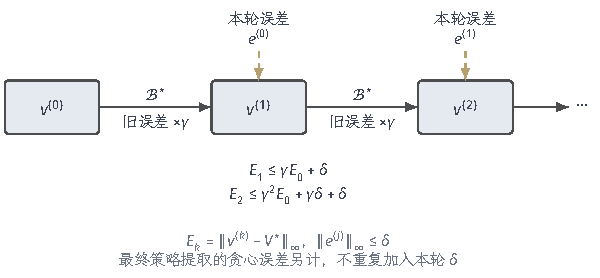
\includegraphics[width=101.533mm]{figures/07-reinforcement-learning/01-problems-and-solving/tikz/rl-planning-error-flow.pdf}
 \caption{近似价值迭代的误差传播。横向每经过一次理想Bellman备份，旧误差乘$\gamma$；上方$e^{(k)}$在各轮注入。因此第$j$轮的误差对第$k$轮的贡献按$\gamma^{k-1-j}$衰减，而每轮都持续注入的误差不会消失。}
 \label{fig:rl-planning-error-flow}
\end{figure}

\begin{theorem}[近似价值迭代的统一误差界]
 \label{thm:rl-planning-avi-error}
 设时间齐次MDP的状态动作有限、各动作集非空、奖励有界，且$0\leq\gamma<1$，$V^*$为最优折扣价值。给定$\delta\geq0$及状态函数序列$(v^{(k)})_{k\geq0}$，若每轮满足$\lVert v^{(k+1)}-\mathcal B^*v^{(k)}\rVert_\infty\leq\delta$，则
 \begin{equation}
 \lVert v^{(k)}-V^*\rVert_\infty
 \leq\gamma^k\lVert v^{(0)}-V^*\rVert_\infty
       +\frac{\delta(1-\gamma^k)}{1-\gamma}.
 \label{eq:rl-planning-avi-error}
 \end{equation}
 若输出策略$\pi^{(k)}$对$v^{(k)}$的贪心误差不超过$\eta$，其真实性能满足
 \[
 \lVert V^*-V^{\pi^{(k)}}\rVert_\infty
 \leq\frac{2\gamma\lVert v^{(k)}-V^*\rVert_\infty+\eta}{1-\gamma}.
 \]
\end{theorem}
\begin{proof}
 记$E_k=\lVert v^{(k)}-V^*\rVert_\infty$。插入$\mathcal B^*v^{(k)}$并使用压缩性，
 \[
 E_{k+1}\leq
 \lVert v^{(k+1)}-\mathcal B^*v^{(k)}\rVert_\infty+
 \lVert \mathcal B^*v^{(k)}-\mathcal B^*V^*\rVert_\infty
 \leq\delta+\gamma E_k.
 \]
 连续代入得到
 $E_k\leq\gamma^kE_0+\delta\sum_{j=0}^{k-1}\gamma^j$，计算几何和即为第一式。

 提取策略时，插入$\mathcal B^*v^{(k)}$及$\mathcal B^{\pi^{(k)}}v^{(k)}$，两者差至多$\eta$。其余两项分别用最优算子和策略算子的压缩性控制，得到
 \[
 \lVert V^*-V^{\pi^{(k)}}\rVert_\infty
 \leq 2\gamma E_k+\eta+
       \gamma\lVert V^*-V^{\pi^{(k)}}\rVert_\infty.
 \]
 移项即得第二式；$\eta=0$时正好回到精确贪心性能界。
\end{proof}

在教学参数$\gamma=0.9$、每轮统一误差$\delta=0.001$下，几何累积给出渐近价值误差上界$0.01$，再转成精确贪心策略的损失上界为$0.18$。误差先在价值迭代中累积，又在长期执行的性能比较中放大；两个分母各有来源。这些是可能保守的解析上界，不表示实际网格正好损失相应数值。

上界使用最大状态误差，而拟合目标可能只控制加权二范数，两种精度不能直接交换。假设一个状态在拟合分布中仅有$10^{-6}$概率，误差为1，其他状态误差为0，加权二范数仍只有$10^{-3}$。部署若恰好从这个状态开始，低权重下的小误差指标就没有控制初始决策。要将加权误差转成性能界，还需限制部署占用相对拟合分布的偏移，例如要求覆盖并控制密度比，即同一状态在两分布中的概率之比。原分布给零概率的状态，也不能靠增加该分布上的样本数覆盖。生成模型下拟合价值迭代的有限时间分析因此保留函数类的逼近能力，以及相关未来状态分布相对拟合分布的密度比控制条件。具体控制哪些未来状态分布、怎样聚合它们的密度比，取决于所用的误差传播界，不能只检查最终策略的一份占用分布\scite{rl2-munos2008-fitted}

近似策略迭代每轮评价的是一份变化中的策略，不是直接近似一次$\mathcal B^*$更新，所以式~\eqref{eq:rl-planning-avi-error}~的假设不再对应。我们改为控制每轮估值离当前策略真实价值的最大误差。若
$\lVert v^{(k)}-V^{\pi^{(k)}}\rVert_\infty\leq\varepsilon$，
改进误差不超过$\eta$，则
$\mathcal B^{\pi^{(k+1)}}V^{\pi^{(k)}}\geq \mathcal B^*V^{\pi^{(k)}}-\beta
\geq V^{\pi^{(k)}}-\beta$，
其中$\beta=2\gamma\varepsilon+\eta$。比较$\mathcal B^*v^{(k)}$与$\mathcal B^{\pi^{(k+1)}}v^{(k)}$给出$\eta$，把两边估值换回真实$V^{\pi^{(k)}}$各付出至多$\gamma\varepsilon$，便得到这项不等式。
为把一次可能下降的备份转成新策略真实价值的下降界，利用恒等式
\[
 V^{\pi'}-V^\pi
 =(\bm I-\gamma\bm T^{\pi'})^{-1}(\mathcal B^{\pi'}V^\pi-V^\pi)
\]
这里$\pi=\pi^{(k)}$、$\pi'=\pi^{(k+1)}$。逆矩阵的几何级数非负，行和为$1/(1-\gamma)$，因而备份下降至多$\beta$时，真实价值满足$V^{\pi'}\geq V^\pi-\beta/(1-\gamma)$。
再比较新策略与最优价值，在两者之间插入$\mathcal B^*V^\pi$和$\mathcal B^{\pi'}V^\pi$，逐状态得到
\[
\begin{aligned}
 V^*-V^{\pi'}
 &=\mathcal B^*V^*-\mathcal B^{\pi'}V^{\pi'}\\
 &\leq\gamma\lVert V^*-V^\pi\rVert_\infty
       +\beta+\gamma\bm T^{\pi'}(V^\pi-V^{\pi'})\\
 &\leq\gamma\lVert V^*-V^\pi\rVert_\infty+\frac{\beta}{1-\gamma}.
\end{aligned}
\]
由于$V^*\geq V^{\pi'}$，对状态取最大值得到保守递推
$\lVert V^*-V^{\pi^{(k+1)}}\rVert_\infty
\leq\gamma\lVert V^*-V^{\pi^{(k)}}\rVert_\infty+\beta/(1-\gamma)$，
将这项递推展开为几何和，渐近损失至多$\beta/(1-\gamma)^2$。这里控制的是每轮相对\emph{当前策略真实价值}的评价误差；AVI，即近似价值迭代，控制的则是一次最优备份误差，二者不能混用。更细的加权范数和不同迭代安排的误差传播可见Farahmand等\scite{rl2-farahmand2010-errors}

% Outline: 2.6
\section{可计算性与复杂度边界}
\label{sec:rl-planning-complexity}

同样一步Bellman备份，背后的实际代价可能天差地别：有的是对一行已知概率逐项求和，有的要反复采样，连续动作还要调用数值优化器。它们写在伪代码里可能都只是“一行更新”，但若不统一计量单位，就无法判断一个算法究竟快还是慢。沿用前面的精确表项、解析动力学或生成模型访问协议，可以分别计算各种方法为了求得价值表、策略或根动作及相应精度所需要的算术运算、存储空间与模型查询次数；只有这些单位先固定下来，“迭代次数少”或“复杂度与状态数无关”这类说法才有确切含义。

% Outline: 2.6.1
\subsection{复杂度指标与模型访问}
\label{sec:rl-planning-access-complexity}

为了比较“一次完整扫描”和“一棵采样树”的代价，先要分清四类资源各计什么。\term{算术运行时间}数加法、乘法等基本运算的次数，回答计算量多大；\term{存储复杂度}数同一时刻需要同时保留的模型、价值、策略和搜索节点，回答要占多少内存；\term{并行深度}数即便有无限多个处理器、仍然必须按顺序完成的依赖层数，回答并行之后最快能多快；\term{模型调用复杂度}则数向外部模型接口发起查询的次数，回答要消耗多少（往往昂贵的）仿真或真实采样。增加处理器可以在依赖允许的范围内缩短延迟，却不会自动减少总运算量或总样本数。

表~\ref{tab:rl-planning-access-models}~对应四种模型表示的基本操作。读取一个表项、遍历一个后继集合和取得一个随机样本，返回的转移概率、后继值或单次奖励记录不同；因此必须先规定一次访问指什么，再比较调用次数。

\begin{table*}[htbp]
 \centering
 \small
 \begin{tabularx}{\linewidth}{@{}l>{\raggedright\arraybackslash}X>{\raggedright\arraybackslash}X@{}}
  \toprule
  模型表示 & 基本访问操作 & 一次备份仍需付出的代价\\
  \midrule
  显式稠密转移表 & 读取一个概率或奖励表项 & 对$n_S$个后继求和；需要整个模型的存储\\
  稀疏转移表 & 遍历一个状态动作的非零后继 & 对$b$个后继求和，并读取对应价值\\
  解析动力学 & 计算状态转移或积分表达式 & 单次函数代价依公式而定；有公式不等于积分可解析\\
  生成模型 & 给定$(s,a)$取得一个独立$(r,s')$ & 用样本均值估计期望；还须计样本数与失败概率\\
  \bottomrule
 \end{tabularx}
 \caption{不同模型访问协议的计数单位。表中$b$表示非零后继数；生成模型的一次查询通常只产生一个后继，不能与遍历整行概率等价计数。}
 \label{tab:rl-planning-access-models}
\end{table*}

以同一个后继期望$T_av$为例，稀疏精确模型要读取$b$个后继价值并加权求和，没有采样误差。生成模型用$m$个后继样本的均值近似它，调用代价随$m$增加，精度则要附带失败概率。即使$m<b$，也只是以更少查询换取近似结果；比较同精度下的速度，还要说明两者误差标准如何对齐。

所求价值表、策略或根动作的精度要求也要固定。全状态价值精度约束每个坐标，给定$\mu_0$的策略精度约束其回报差，当前状态选择则只需控制一个根决策的损失。三者不同，不能共用所有下界：写出$n_S$维显式价值表本身至少需要$\Omega(n_S)$次写入，而输出一个根动作不需要写出这张表。

一次基本算术运算按单位成本计数，前提是将参与运算的数视为可在单步处理。模型编码的读取、价值表或策略等结果的表示长度，以及运算数目分别给出资源要求，不能用迭代次数代替全部成本。若进一步计算位复杂度，即处理数字的二进制编码所需的工作，还要考虑转移概率的编码位长、目标精度和精确消元中的分子分母增长。多项式算术步数并不意味着每一步的位运算都只需常数成本；采用浮点实现时，舍入误差也应纳入残差证书。

% Outline: 2.6.2
\subsection{全状态动态规划的计算代价}
\label{sec:rl-planning-dp-complexity}

先数一次精确最优Bellman扫描的工作。设状态数为$n_S$，每处合法动作至多$n_A$，实际状态动作对的平均非零后继数为$b$。扫描逐个状态枚举动作，再遍历各动作的后继；状态动作对至多$n_Sn_A$个，每对平均付出$b$次后继计算，因此代价上界为
\begin{equation}
 O(n_Sn_Ab).
 \label{eq:rl-planning-sweep-cost}
\end{equation}
若转移稠密，$b=n_S$，一次扫描便为$O(n_S^2n_A)$。稀疏模型及奖励占$O(n_Sn_Ab)$存储，价值表占$O(n_S)$；确定性策略每状态只存一个动作索引，共$O(n_S)$个字，随机策略则至多存$O(n_Sn_A)$个概率。同步更新多留一张价值表，但价值存储阶仍为$O(n_S)$，模型存储要另外计入。

总运行时间还要乘扫描轮数。压缩性给出第$k$轮误差至多$\gamma^kE_0$，其中$E_0$界住初始误差；要使它不超过$\varepsilon$，在$0<\gamma<1$、$0<\varepsilon<E_0$时解这个不等式，得到充分轮数
\begin{equation}
 k\geq\left\lceil\frac{\log(E_0/\varepsilon)}{-\log\gamma}\right\rceil.
 \label{eq:rl-planning-iteration-count}
\end{equation}
从零初始化时，有界回报给出$E_0=R_{\max}/(1-\gamma)$。利用$-\log\gamma\geq1-\gamma$，可以进一步采用较保守的
$O((1-\gamma)^{-1}\log(E_0/\varepsilon))$轮数上界。$\gamma$越接近1，未来影响衰减越慢，达到同一精度可能需要更多轮。边界也要分开：$\gamma=0$时一次备份已最优，$\varepsilon\geq E_0$时初值已满足精度，都无须使用对数式。

表~\ref{tab:rl-planning-dp-costs}~将各操作的单轮成本与轮数要求分开。固定确定性策略只使用一个动作，稠密随机策略还要按动作概率混合，或提前构造$\bm T^\pi,\bm r^\pi$。若直接解稠密$n_S$阶评价方程，常规消元需$O(n_S^3)$运算及$O(n_S^2)$存储。稀疏消元可能产生填充，即原本为零的位置在消元中变成非零，所以不能仅将$b$代入稠密立方公式，就认定得到稀疏求解代价。

\begin{table*}[htbp]
 \centering
 \small
 \begin{tabularx}{\linewidth}{@{}l>{\raggedright\arraybackslash}X>{\raggedright\arraybackslash}X@{}}
  \toprule
  操作 & 单轮算术代价 & 轮数或输出条件\\
  \midrule
  固定确定性策略的迭代评价 & 一次固定策略扫描$O(n_Sb_\pi)$ & $b_\pi$为所选动作平均后继数；轮数由评价压缩或残差确定\\
  策略改进 & $O(n_Sn_Ab)$ & 只比较一次动作；不包括评价\\
  价值迭代 & $O(n_Sn_Ab)$ & 达到价值误差的轮数见式~\eqref{eq:rl-planning-iteration-count}\\
  精确策略迭代 & 稠密评价$O(n_S^3)$加改进；模型混合另计 & 外层轮数依问题而变；有限终止论证只给有限策略数的粗界\\
  \bottomrule
 \end{tabularx}
 \caption{全状态动态规划的成本。$b_\pi$可能与所有动作平均的$b$不同；表中随机策略若未预先混合转移，评价扫描还需计入动作枚举。}
 \label{tab:rl-planning-dp-costs}
\end{table*}

前面的有限终止证明只用到了确定性策略总数$\prod_s|\mathsf A(s)|$。它对$n_S$可能指数增长，因此既不是紧的轮数分析，也不是多项式时间结论。若要作更细比较，必须说明策略迭代的具体规则、折扣是否固定，以及复杂度定理所计的模型编码规模与运算。

同步扫描内，各状态动作的后继求和可以并行。令$b_{\max}$为最大非零后继数，树状求和再比较动作最大值的依赖深度为$O(\log(1+b_{\max})+\log(1+n_A))$；这里必须用最大值而不是平均$b$，因为并行延迟由最长计算链决定。第$k+1$轮仍使用第$k$轮的价值，所以有足够处理器也不能将所有轮次同时完成。

% Outline: 2.6.3
\subsection{时域、分支与搜索复杂度}
\label{sec:rl-planning-search-complexity}

局部搜索省去了全状态扫描，却可能反复展开同一位置的不同历史。为数完整树的规模，固定每处$A$个动作、每个动作$B$个随机后继，并以动作执行次数计深度$H$。每层状态节点增加$AB$倍，因此状态节点总数为
$\sum_{h=0}^{H}(AB)^h$，非叶状态处的动作节点数为
$A\sum_{h=0}^{H-1}(AB)^h$。
当$AB>1$时，前者为$[(AB)^{H+1}-1]/(AB-1)$，随深度指数增长；$AB=1$时则只有一条长度$H$的链，不能使用分母为0的几何和形式。

若两条历史到达同一网格位置，且剩余步数相同，马尔可夫性保证它们面对同一个后继子问题。于是可合并相同的$(s,\text{剩余深度})$，用动态规划图复用结果；连终端层在内至多有$(H+1)n_S$个时层状态，其中至多$Hn_S$个需要备份。合并要支付状态识别与存储成本，利用的是当前状态与剩余步数对后继子问题的充分性，而非删除真实随机后果。连续状态很少精确重复时，这种复用可能收益有限。

表~\ref{tab:rl-planning-search-costs}~回到同一棵搜索树，比较截断、采样、叶值、自适应访问和状态合并各省去什么工作。稀疏采样将每动作后继数$B$替换为$m$，仍保留$(Am)^H$的深度依赖；MCTS只展开访问到的节点，但减少节点不等于普遍改善固定预算下的最坏决策误差。

\begin{table*}[htbp]
 \centering
 \small
 \begin{tabularx}{\linewidth}{@{}l>{\raggedright\arraybackslash}X>{\raggedright\arraybackslash}X@{}}
  \toprule
  手段 & 减少的计算 & 误差及额外条件\\
  \midrule
  深度截断 & 删除$H$步之后的展开 & 尾和或$\gamma^H\varepsilon$终端误差；短视不可逆动作仍危险\\
  稀疏采样 & 每个动作只抽$m$个后继 & 样本均值及递归误差；独立生成模型、置信度和树规模\\
  叶值近似 & 用一次求值替代叶外模拟 & 叶值必须在到达区域准确；预计算和训练代价另计\\
  MCTS & 将查询集中于被选择的分支 & 回报非平稳、叶值偏差与探索条件；选择性展开不是普遍最坏界\\
  状态合并 & 复用相同状态及剩余深度的计算 & 要求状态表示足以确定剩余决策问题的转移与奖励规律，并支付索引与存储成本\\
  \bottomrule
 \end{tabularx}
 \caption{搜索预算的节省对象。不同手段可以组合，但组合后的误差应按实际接口重新分析。}
 \label{tab:rl-planning-search-costs}
\end{table*}

若一次MCTS模拟至多走$H$层，每层只抽一个后继，叶值评估又需$L$次模型调用，则调用至多为$H+L$，$N$次模拟至多为$N(H+L)$。这个计数不含动作枚举、网络求值或连续优化，也没有说明误差随$N$减小多快。模拟长度随机时，还应分别报告期望调用和尾部延迟；平均用时小于预算不保证每次都在截止时间内返回。

% Outline: 2.6.4
\subsection{计算下界}
\label{sec:rl-planning-lower-bounds}

前面给出的都是上界：我们构造了某个算法，并数清它需要多少工作。但上界无法回答“还能不能更省”。要证明某类问题在给定接口下至少要付出多少代价，常用的办法是构造\term{不可区分问题对}：设置两个环境，让它们对算法已经发起的查询返回相同记录，却在尚未查询的奖励表项或后继分支上有所不同，使真正的最优动作也不同。只凭这份共同记录，算法无法确定自己面对哪一个环境；若必须在两者中都精确选对，就须继续取得能够区分它们的查询记录。对允许随机失败的算法，则要控制两环境下查询记录分布的差别及相应的判别错误概率。这样才能分别得到精确表项读取和随机样本辨识的资源下界。

先隔离精确表项的读取代价。一个单步问题有$n_A$个动作，算法已读奖励都为0，未查动作中可能有一个奖励为1。若还剩至少两个未查动作，就可以分别把唯一奖励1放在它们上面，得到相同读取记录和不同最优动作。因此要求精确最优的确定性算法，最坏至少要查$n_A-1$个表项；扫描全表给出$O(n_A)$上界。奖励没有随机性，取得未查动作的奖励值仍须付出读取成本。

换成生成模型，一次读到的奖励不再确定其期望，我们就要数样本辨识的代价。考虑单状态、单步、两动作，即$H=1$、没有后续奖励，也等价于$\gamma=0$。奖励在$[0,1]$内，动作$a_1$恒得$1/2$，动作$a_2$在模型$M_+$和$M_-$中分别服从
$\operatorname{Bernoulli}(1/2+2\varepsilon)$和
$\operatorname{Bernoulli}(1/2-2\varepsilon)$，其中$0<\varepsilon\leq1/8$。
要求算法输出一个确定性根动作，并在模型样本及自身随机性下，以至少$1-\alpha$的概率使该动作期望奖励离最优不超过$\varepsilon$，其中$0<\alpha<1/4$。两模型的最优动作相反，选错会损失$2\varepsilon$，所以达到精度要求就必须分辨它们。

为计算自适应奖励查询积累的对数似然证据，令$T$为停止查询的时刻，$A_k,X_k$为第$k$次查询的动作与奖励，$\widehat a$为最终根动作。完整记录包含独立于环境的内部随机种子，以及$(A_k,X_k)_{k=1}^T$、$T$和$\widehat a$；记它在两模型下的分布为$\mathbb P_+,\mathbb P_-$。要求$T$在两模型下几乎必然有限；若$\mathbb E_+N_2=\infty$，下界已经成立，下面只需考虑有限期望，其中$N_2=\sum_{k=1}^T\mathbf1\{A_k=a_2\}$。记录分布的KL仍是按前一分布平均对数似然比，即$D_{\mathrm{KL}}(\mathbb P_+\Vert\mathbb P_-)=\mathbb E_+\log(d\mathbb P_+/d\mathbb P_-)$，其中$d\mathbb P_+/d\mathbb P_-$表示同一记录在两模型下的似然比。

给定同一已有历史，同一个算法的动作选择、停止和输出规则相同，内部种子的分布也相同，因此这些因素在记录似然比中相消。$a_1$的奖励在两模型下相同，也不贡献；只有每次$a_2$的奖励留下一个似然比。令$p=1/2+2\varepsilon$、$q=1/2-2\varepsilon$，$f_p,f_q$为相应Bernoulli概率质量函数，下面将Bernoulli分布简记为$\operatorname{Ber}$。于是
\[
 \begin{aligned}
 \log\frac{d\mathbb P_+}{d\mathbb P_-}
 &=\sum_{k=1}^{T}\mathbf1\{A_k=a_2\}
          \log\frac{f_p(X_k)}{f_q(X_k)},\\
 D_{\mathrm{KL}}(\mathbb P_+\Vert\mathbb P_-)
 &=\mathbb E_+N_2\,
       D_{\mathrm{KL}}(\operatorname{Ber}(p)\Vert\operatorname{Ber}(q)).
 \end{aligned}
\]
第二式先对每次查询前的历史取条件期望，再对查询次数求和；这里单次对数比有界，$\mathbb E_+N_2$有限，保证求和与期望可交换。停止时间下的这类换测度等式见Kaufmann等附录A式(18)\scite{rl3-kaufmann2016complexity}

利用$\log z\leq z-1$分别界住Bernoulli散度的两项，可得
\[
 \begin{aligned}
 D_{\mathrm{KL}}(\operatorname{Ber}(p)\Vert\operatorname{Ber}(q))
 &\leq\frac{(p-q)^2}{q(1-q)}
 \leq\frac{256}{3}\varepsilon^2.
 \end{aligned}
\]
最后一步使用$p-q=4\varepsilon$、$q\in[1/4,1/2)$和$q(1-q)\geq3/16$。取$C=256/3$，总记录散度便至多为$C\varepsilon^2\mathbb E_+N_2$，这说明每个样本能积累的分布差别很少。

再以事件$B=\{\widehat a=a_1\}$把输出看作二元检验：$\mathbb P_+(B)$和$\mathbb P_-(B^{\mathrm c})$分别是两模型中的错误概率。两种Bernoulli参数均在$(0,1)$内，奖励支持相同；结合共同的算法规则及两模型下有限的$T$，记录分布互相绝对连续，即任一记录事件在一个模型下概率为0时，另一个也为0。在此条件下，检验界给出
\[
 \mathbb P_+(B)+\mathbb P_-(B^{\mathrm c})
 \geq\tfrac12\exp[-D_{\mathrm{KL}}(\mathbb P_+\Vert\mathbb P_-)].
\]
这里使用Kaufmann等附录A引理20中的事件形式\scite{rl3-kaufmann2016complexity}
成功要求使左侧不超过$2\alpha$，故记录散度至少为$\log(1/(4\alpha))$。与上界合并，得到
\[
 \mathbb E_+N_2\geq
 \frac{\log(1/(4\alpha))}{C\varepsilon^2}.
\]
这说明记录必须积累足够的分布差别，才能达到规定的检验成功率。对$\alpha\leq1/8$，所需样本阶为
$\Omega(\varepsilon^{-2}\log(1/\alpha))$。反过来，用固定次数独立样本估计$a_2$均值，与$1/2$比较，Hoeffding不等式给出同阶上界。若接口直接返回精确期望，只查一次就能区分二者，这条样本下界随即不适用。

再将困难放在未查搜索分支中，而不是奖励采样中。考虑深度$H$、每层$n_A\geq2$动作的完整确定性树，目标有限时域且不折扣。此前奖励都为0，$n_A^H$个终端叶子中恰有一个得1，其余为0；结构已知，但只能逐次精确查询叶奖励，没有可利用的参数关系或内部节点摘要。要求以至少$2/3$概率输出损失不超过$\varepsilon<1/2$的确定性根动作，也就是选中包含奖励叶的根分支。

若把唯一奖励叶在$n_A^H$个位置均匀放置，至多$q$次查询发现它的概率不超过$q/n_A^H$。固定算法的随机种子后，在所有查询都返回0的记录上，算法只能输出某个根分支；该分支最多包含全部叶子的$1/n_A$，所以“未发现且猜对”这一联合事件的概率至多为$1/n_A$。对随机种子取平均，界仍成立。因此总体成功率不超过$q/n_A^H+1/n_A$，要达到$2/3$，必有$q\geq n_A^H/6$。这个对奖励叶位置均匀抽样的论证，也推出至少一种奖励叶配置上的随机算法预算下界；扫描全部叶子则给匹配上界。指数困难来自没有结构的叶奖励表，不能把它推广为所有简洁模型的不可解性，或声称共享状态的网格必然需要同样多的查询。

表~\ref{tab:rl-planning-bounds}~分别将三个受限问题族的下界与同条件上界并列。每行数量级匹配，含义是该行指定任务所需资源的阶已确定；行间接口、精度和成功概率不同，不能合并为一般MDP的统一最优复杂度。

\begin{table*}[htbp]
 \centering
 \small
 \begin{tabularx}{\linewidth}{@{}>{\raggedright\arraybackslash}Xcc>{\raggedright\arraybackslash}X@{}}
  \toprule
  问题配置、目标与查询接口 & 下界 & 同条件上界 & 匹配范围\\
  \midrule
  单步$n_A$动作、精确奖励表、精确最优动作 & $\Omega(n_A)$ & $O(n_A)$ & 表项读取次数，不是随机样本数\\
  单步两动作Bernoulli模型、$\varepsilon\leq1/8$、$\alpha\leq1/8$ & $\Omega(\varepsilon^{-2}\log(1/\alpha))$ & $O(\varepsilon^{-2}\log(1/\alpha))$ & 独立生成样本；常数因子未追求一致\\
  完整确定树、唯一奖励叶、根动作成功率$2/3$ & $\Omega(n_A^H)$ & $O(n_A^H)$ & 精确叶奖励查询；不含到叶路径执行成本\\
  \bottomrule
 \end{tabularx}
 \caption{三个受限问题族中的上、下界。它们分别隔离奖励表项读取、统计辨识和搜索宽深度，不能合并为一个适用于所有MDP的复杂度公式。}
 \label{tab:rl-planning-bounds}
\end{table*}

两臂下界还没有说明一般有限MDP的状态数和长期传播怎样影响采样。考虑$n_S$个状态、每个状态$n_A$个动作的时间齐次折扣MDP，$0<\gamma<1$，奖励为已知确定性函数$R(s,a)\in[0,1]$。生成模型允许在任意指定的$(s,a)$独立采样后继；对每对查询$N$次，以后继计数的频率构造经验转移$\widehat T$，便得到一份可交给前面规划算法的经验MDP。用$\widehat V^\pi$和$\widehat V^*$表示该经验模型中的策略价值和最优价值，区别于真实环境中的$V^\pi,V^*$。

采样后不能只证明某份预先固定策略的估值准确，因为规划器会主动选择在这批记录上看起来最好的策略。Agarwal等处理了所选策略与经验转移之间的依赖，得到如下代表性样本保证：对$\varepsilon\in(0,1]$、$\delta\in(0,1)$，存在通用常数$c,C>0$，当
\begin{equation}
 \begin{aligned}
 N&\geq\max\left\{1,
   \frac{c\log\!\bigl(8n_Sn_A/[(1-\gamma)\delta]\bigr)}
        {(1-\gamma)^3\varepsilon^2}\right\},\\
 \|\widehat V^*-\widehat V^{\widehat\pi}\|_\infty
      &\leq\varepsilon_{\mathrm{opt}}
       \leq(1-\gamma)\varepsilon,
 \end{aligned}
 \label{eq:rl-planning-generative-rate}
\end{equation}
达到右侧精度的合法平稳策略$\widehat\pi$，以至少$1-\delta$的概率满足
$\|V^*-V^{\widehat\pi}\|_\infty\leq C\varepsilon$。
这里概率针对生成查询，内部规划器须确实达到所列全状态精度。这个状态价值结论需要保留动作选择的质量，不能仅由$Q^{\widehat\pi}$接近$Q^*$直接改写出来。取真实最优策略$\pi^*$，用$\widehat Q^\pi$表示同一策略在经验模型中的动作价值，则
\[
 \|V^*-V^{\widehat\pi}\|_\infty
 \leq \|Q^*-\widehat Q^{\pi^*}\|_\infty
       +\varepsilon_{\mathrm{opt}}
       +\|\widehat Q^{\widehat\pi}-Q^{\widehat\pi}\|_\infty.
\]
这是在两份真实价值之间插入$\widehat V^{\pi^*}$和$\widehat V^{\widehat\pi}$所得：首末两项比较同一策略在两个模型中的价值，可按该策略平均动作价值误差；中项由$\widehat V^{\pi^*}\leq\widehat V^*$及规划精度控制。强的经验状态价值条件也保证
$\|\widehat Q^*-\widehat Q^{\widehat\pi}\|_\infty
\leq\gamma\varepsilon_{\mathrm{opt}}$。
原分析同时控制上式首末两个动作价值估计误差，按所列$N$与内部精度即可得到$C\varepsilon$界；保留中项避免漏掉初始动作选错的损失。

按式\eqref{eq:rl-planning-generative-rate}左侧阈值的数量级选择正整数$N$，总查询数为$n_Sn_AN$，因而在隐藏对数因子的记法下为
$\widetilde O\!\left(n_Sn_A/[(1-\gamma)^3\varepsilon^2]\right)$；
将$\varepsilon$按常数缩小即可得到预先指定的策略误差。内部精度也随$1-\gamma$缩小，因为经验规划误差会通过后续执行放大\scite{rl2-agarwal2020-generative}

这条结果不要求先将整张转移表逐项估到很小的总变差。分析利用后继价值的方差，并通过将一个状态改为吸收状态的辅助模型，解除待评价价值与该状态转移样本之间的部分依赖；只对固定函数套一次集中界不够。经验模型随后可以调用价值迭代或其他达到所需精度的规划器，所以同一个外部样本率可以对应不同的内部运算和存储开销。极小极大率比较指定MDP类中最不利环境的样本需求，不等于每个具体网格都同样困难，也不是精确概率表的读取下界。真实在线交互通常还不能查询未到达状态，还须承担探索与可达性的代价。

% Outline: 2.7
\section{本章小结}
\label{sec:rl-planning-summary}

章首的问题现在可以分成两步回答：准确模型给出了计算长期后果的依据，所求价值表、策略或根动作及预算决定我们能算到哪里。在基准网格上，精确Bellman求解和占用量线性规划都得到同一个最优起点价值
$J(\pi^*)\approx0.421161$；前文定义并评价的均匀合法策略满足
$J(\pi_{\mathrm u})\approx-0.154754$。最优策略与均匀合法策略的回报差来自行动方式，而不是更换奖励或滑移规则。价值评价各状态的长期后果，占用量记录策略怎样分配折扣时间；二者由
$J(\pi)=(1-\gamma)^{-1}\sum_{s,a}d^\pi(s,a)R(s,a)$联系，所以归一化流量恢复为未归一化回报时，必须保留尺度系数。

进一步减少精确计算，要找到实际模型中的结构，而不是只辨认方法名称。LQR用动力学与成本保持二次价值，KL控制用受限转移和偏离费用使方程换元线性化；递减差分支持单调选择，独立子过程还须配合笛卡尔积动作才能直接分解。它们可以叠加，但动作约束、噪声机制或共享资源的改变也可能破坏原推导，使用时应回到对应条件检查。

资源仍不足时，可以局部搜索，也可以保存可复用的近似价值，二者能在叶值处结合。表~\ref{tab:rl-planning-method-choice}~按所求价值表、策略或根动作、模型访问协议和资源归纳这种选择，并列出应检查的误差依据。深度限制留下尾部误差，有限样本留下期望估计误差，函数表示与拟合留下跨状态误差，动作求解还可能留下选择误差；减小其中一项并不自动减小其他项。

\begin{table*}[htbp]
 \centering
 \small
 \begin{tabularx}{\linewidth}{@{}l>{\raggedright\arraybackslash}X>{\raggedright\arraybackslash}X>{\raggedright\arraybackslash}X@{}}
  \toprule
  所求决策对象 & 模型接口与资源 & 可用方法 & 应报告的证书或边界\\
  \midrule
  全状态精确价值／策略 & 精确期望，可存表并扫描 & 动态规划、价值或占用LP & 全状态残差、原对偶间隙及恢复条件\\
  特殊结构的反馈律 & 解析模型，结构满足假设 & Riccati、线性换元、阈值或分解 & 封闭、可稳定、差分或独立性条件\\
  当前状态动作 & 精确展开，在线时间有限 & 有限前瞻与滚动规划 & 截断尾界、叶值误差、根动作与执行损失的区别\\
  当前状态动作 & 独立生成样本，调用预算有限 & 稀疏采样、MCTS & 查询次数、置信度、叶值与探索条件\\
  可复用的全状态近似 & 精确或采样模型，价值表过大 & 聚合、拟合评价、近似策略／价值迭代 & 一致误差界；若只有加权误差，另需覆盖条件\\
  \bottomrule
 \end{tabularx}
 \caption{模型已知时的方法选择。时间与存储应包含预计算、在线求值及模型本身；经验表现不能替代所列条件下的误差保证。}
 \label{tab:rl-planning-method-choice}
\end{table*}

下一章沿用本章的理想Bellman算子、评价与改进关系及性能界，却不再默认能够访问准确模型。学习者还要采集交互训练记录，从中估计价值或环境规律，并处理策略改变后训练记录分布随之改变的问题。某些统计分析会单独保留生成模型假设以隔离估计困难，真实在线学习则通常只能沿实际轨迹采集。于是本章的计算误差，将与统计误差、覆盖和探索共同决定能够得到怎样的策略。
